% !TEX root = main.tex
\chapter{Dữ liệu và phương pháp xây dựng hệ thống}

\section{Tổng quan hệ thống}

\begin{figure}[H]
    \centering
    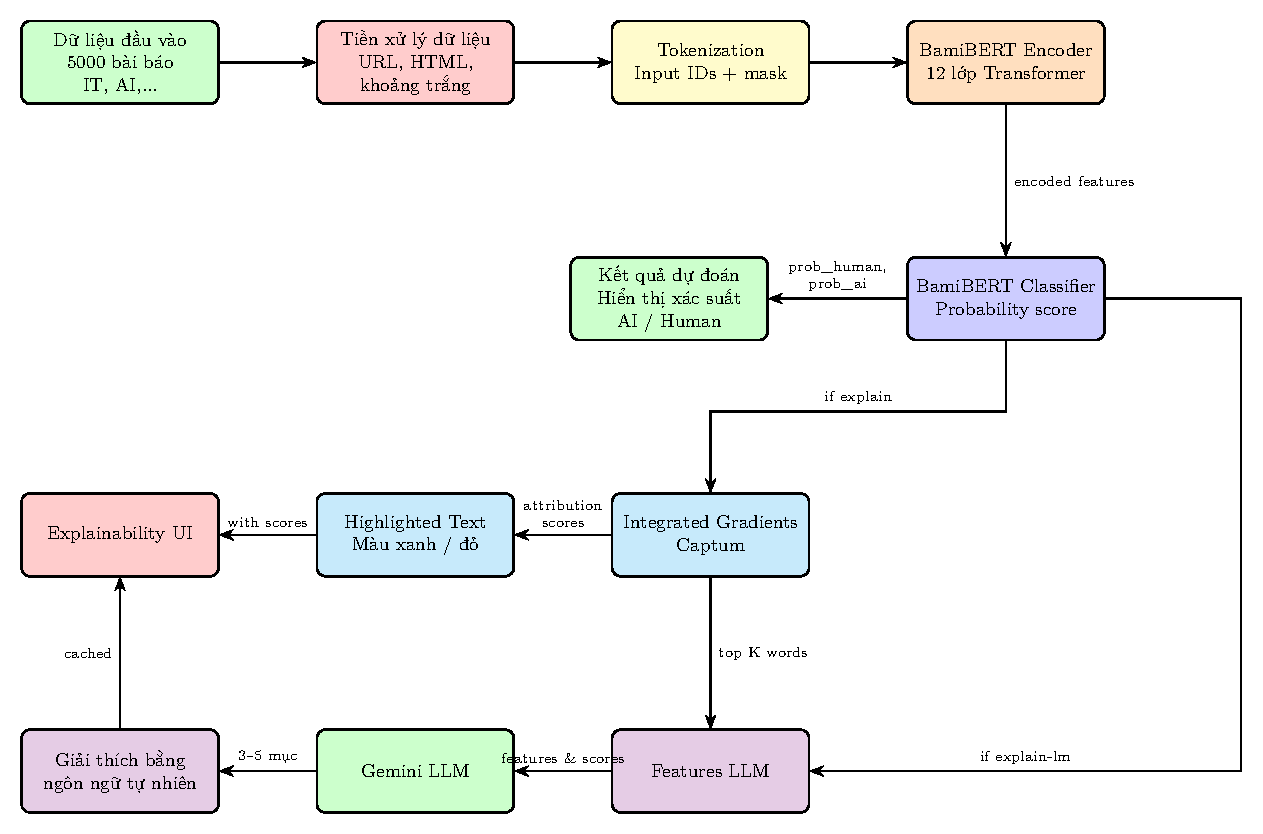
\includegraphics[width=\textwidth]{figures/chapter_03/system_architecture.pdf}
    \caption{Kiến trúc hệ thống}
    \label{fig:system_architecture}
\end{figure}

Trong hệ thống trên, dữ liệu đầu vào tập trung vào các bài báo tiếng Việt chuyên về lĩnh vực công nghệ thông tin (IT), AI hay là các thiết bị công nghệ hiên đại. Dữ liệu sau đó được tiền xử lý bằng cách loại bỏ các URL, HTML, và khoảng trắng thừa, dữ liệu đã được làm sạch
sẽ được đưa vào quá trình token hóa, để ánh xạ mỗi từ sang các chỉ số đầu vào (input IDs) và mặt nạ (mask). Tiếp theo, các token này sẽ được được vào mô hình BamiBERT để embedding, tức là chuyển các token thành các vector đặc trưng rồi bắt đầu quá trình huấn luyện. Đầu ra
của mô hình chính là xác suất dự đoán của văn bản dựa vào hai lớp, Human hay là AI.

\vspace{\baselineskip}
\noindent
Ngoài ra, hệ thống còn có khả năng giải thích kết quả do mô hình dự đoán bằng cách sử dụng thuật toán Integrated Gradients, thuật toán này sẽ tính điểm đóng góp cho từng token của đoạn văn bản, dựa vào điểm đóp góp đó thì hệ thống sẽ hiển thị giao diện bằng cách highlight các từ đó theo
các màu tương ứng với hai lớp, cụ thể màu đó là AI và màu xanh là người viết, độ sáng của các màu thể hiển mức độ đóng góp, ảnh hưởng đối với kết quả dự đoán, màu càng đậm thì càng ảnh hưởng lớn đối với kết quả dự đoán.

\vspace{\baselineskip}
\noindent
Tiếp theo để hệ thống có khả năng giải thích bằng ngôn ngữ tự nhiên, hệ thống đã sử dụng một mô hình LLM, đó là Gemini, với sự ràng buộc yêu cầu (prompt) dựa trên các từ có điểm đóng góp cao từ thuật toán IG, và các chỉ số đo lường ví dụ như mật độ dấu câu, độ dài câu,\dots Sau đó câu lệnh sẽ được mô hình
Gemini xử lý và trả về kết quả giải thích bằng ngôn ngữ tự nhiên, kết quả này sẽ được hiển thị trên giao diện của người dùng.

\section{Thu thập và xây dựng dữ liệu}
\subsection{Nguồn dữ liệu}
Nguồn dữ liệu được thu thập trong đồ án chủ yếu là đến từ các trang báo, bài viết tiếng Việt thuộc lĩnh vực công nghệ thông tin, AI hay các thiết bị công nghệ hiện đại, \dots Việc lựa chọn một lĩnh vực cụ thể nhằm đảm bảo dữ liệu có tính thống nhất về chủ đề, đồng thời hạn chế về sự khác biệt về chủ đề có ảnh hưởng đến quá trình học của mô hình. Ngoài 
ra, lĩnh vực công nghệ có lượng lượng bài báo, nội dung thường xuyên đăng tải liên tục trực tuyến, thường có sự thay đổi về công nghệ, thuật ngữ chuyên môn, tên sản phẩm và tên công nghệ, \dots Điều này tạo nên tính đa dạng về dữ liệu vì cách diễn đạt, cấu trúc bài viết khác nhau.

\begin{figure}[H]
    \centering
    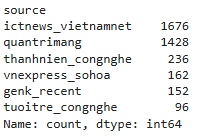
\includegraphics[width=0.4\textwidth]{images/chapter_03/img_13.png}
    \caption{Các nguồn dữ liệu thu thập}
    \label{fig:nlp}
\end{figure}

\vspace{\baselineskip}
\noindent
Phần lớn các bài báo, tin tức được thu thập từ các nguồn uy tín, tên miền rõ ràng, đều là các trang bài báo công nghệ phổ biến ở Việt Nam, bao gồm VnExpress, GenK, Thanh Niên Công Nghệ,\dots Các bài báo được thu thập từ các nguồn này đều có nội dung liên quan đến lĩnh vực công nghệ thông tin, AI hay các thiết bị công nghệ hiện đại,\dots Các nguồn này
được lựa chọn dựa trên mức độ phổ biến, ổn định và độ tin cậy của các trang tin tức Việt Nam. Nhờ vậy mà dữ liệu có nguồn gốc rõ ràng và phù hợp với phạm vi nghiên cứu.


\subsection{Thu thập dữ liệu văn bản Human}
Dữ liệu các bài báo, văn bản Human được thu thập tập trung vào các lĩnh vực công nghệ thông tin, trí tuệ nhân tạo, thiết bị công nghệ hiện đại như đã trình bày ở mục 3.2.1. Mục đích của quá trình này là để xây dựng một bộ dữ liệu bài báo, văn bản được viết và xuất bản bởi con người, lấy làm cơ sở để mô hình học cách phân biệt nội dung giữa con người hay AI tạo ra. Quá trình 
thu thập dữ liệu được tự động hóa bằng cách truy cập các trang tin tức và trích xuất nội dung từ các bài báo, bài viết phù hợp. Đối với mỗi bài viết, các phần quan trọng như URL, nguồn, tên tác giả và ngày xuất bản sẽ được lưu trữ nhằm thể hiện các bài báo đó có nguồn rõ ràng, minh bạch và nội dung của bài báo đó. Các phần không liên quan đến nội dung như quảng cáo, menu hay 
các thành phần giao diện web sẽ được loại bỏ để đảm bảo dữ liệu thu được chỉ tập trung vào các nội dung cần thiết.

\begin{figure}[H]
    \centering
    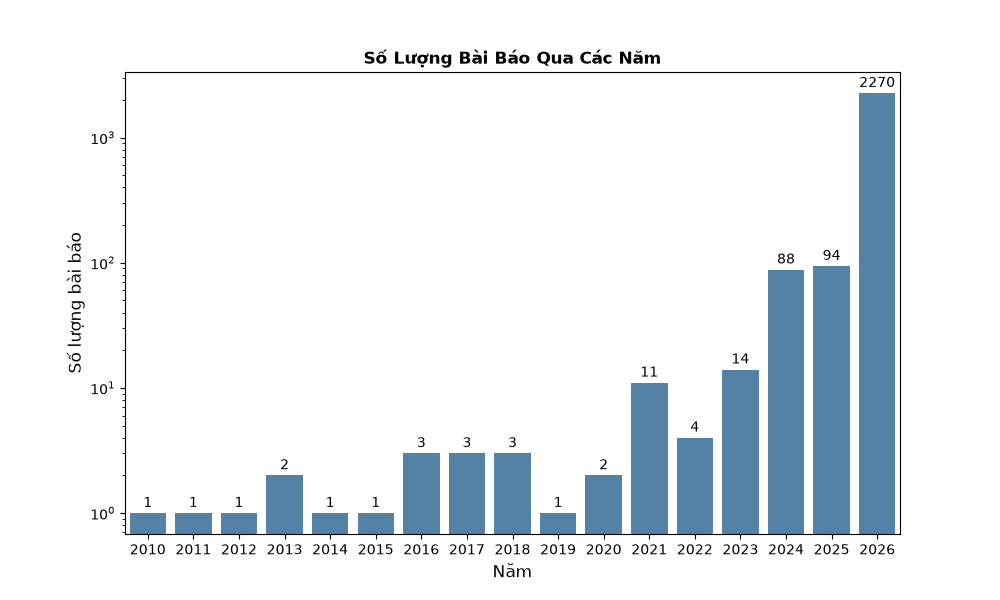
\includegraphics[width=1.0\textwidth]{images/chapter_03/img_14.png}
    \caption{Các bài báo văn bản thu thập qua các năm}
    \label{fig:nlp}
\end{figure}

\vspace{\baselineskip}
\noindent
Như đã thấy ở Hình 14, dữ liệu được thu thập từ các bài báo, tin tức nằm trong khoảng từ năm 2010 cho đến năm 2026 và tập trung hầu hết vào năm 2026 với tổng cộng là 2.270 bài. Nguyên nhân là trong quá trình thu thập dữ liệu, các nguồn tin tức thường cung cấp số lượng bài báo mới hiện nay nhiều hơn so với các bài viết từ các năm trước, ngoài ra thì các bài báo cũ từ các năm trước có 
khả năng truy cập và thu thập bị hạn chế hơn rất nhiều, có thể là do cấu trúc website thay đổi theo thời gian hoặc là do trang lưu trữ dữ liệu các bài báo cũ không còn tồn tại nữa. Do đó, dữ liệu được giữ theo số lượng thực tế thay vì cố gắng thu thập phân bố đồng đều giữa các năm.

\vspace{\baselineskip}
\noindent
Ngoài ra, sẽ có vấn đề là nếu muốn dữ liệu Human là viết hoàn toàn bởi con người, ít ảnh hưởng bởi AI nhất thì tại sao không thu thập dữ liệu từ các năm trước trở xuống, ví dụ như năm 2023, là thời điểm AI chưa phát triển mạnh để các tác giả sử dụng để hỗ trợ khả năng viết bài của họ. Lý do là vì nếu ta chỉ thu thập từ các năm trước, giả sử như năm 2023 trở về trước, thì dữ liệu sẽ bị hạn chế về số lượng 
và tính đa dạng của nó, đó là yếu tổ sự chuyển dịch theo thời gian, giả sử như năm 2023, các bài viết chưa có đề cập đến các chủ đề như Claude, OpenClaw, Gwen, \dots Trong khi các bài báo hiện nay thì lại rất nhiều, điều đó vô tình khiến một vấn đề lớn là khi sau này hệ thống mà triển khai thì khi mà đưa một bài báo mà mô hình chưa thấy chủ đề đó bao giờ thì sẽ khó mà phân loại được, vì bản thân mô hình học sâu,
mô hình được sử dụng trong đồ án ngoài khả năng học cấu trúc câu, thì nó còn học thêm từ vựng, chủ đề và ngữ cảnh xuất hiện trong câu, do đó khả năng tổng quát hóa của mô hình sẽ trở nên kém hơn nếu đem đi triển khai thực tế. Do đó, đồ án quyết định xây dựng dữ liệu qua các năm, từ năm 2010 đến 2026 và tập trung hầu hết từ năm 2024 - 2026 để đảm bảo tính đa dạng về chủ đề, đa dạng hóa các nguồn và sát với dữ liệu
thực tế để đi vận hành triển khai hệ thống. 

\subsection{Xây dựng dữ liệu AI}
Dữ liệu AI được xây dựng dựa trên các mô hình ngôn ngữ lớn (LLM) nhằm tạo ra các mẫu bài báo, văn bản phục vụ cho viết huấn luyện mô hình phân biệt giữa văn bản do con người viết hay AI tạo ra. Dữ liệu bài báo AI được xây dựng bằng cách đưa ra chủ đề kết hợp với yêu cầu hoàn chỉnh để mô hình LLM tạo ra các bài báo, tức là sẽ chọn các chủ đề liên quan đến lĩnh vực đồ án, ví dụ như trí tuệ nhân tạo, smartphone, ứng dụng công nghệ, \dots Sau
đó, đưa ra các yêu cầu cụ thể về độ dài, cấu trúc bài viết, số lượng đoạn văn để đảm bảo giống như các bài báo từ con người, có nguồn rõ ràng để cho mô hình LLM sinh ra. 

\vspace{\baselineskip}
\noindent
Ở phạm vi đồ án, mô hình LLM sử dụng là bao gồm Gemini và DeepSeek, vì lý do là khi sử dụng các mô hình khác, ví dụ như ChatGPT hay Claude thì sẽ tốn token và tốn rất nhiều chi phí mà ngân sách thì hạn hẹp cho nên lựa chọn hai mô hình đó để sinh bài báo, văn bản là cách tối ưu
cho phạm vi đồ án. Tuy vậy, vẫn có một nhược điểm đó là nếu giới hạn các mô hình sinh văn bản như vậy thì khi mà triển khai thì người dùng vẫn có thể sử dụng các mô hình ngôn ngữ khác tốt hơn để sinh bài báo, ví dụ như các mô hình Opus 5 hay Fable 5 của Claude với khả năng viết lách giống như con người hơn thì hệ thống sẽ vẫn khó để phân biệt loại bài báo đó là do con người hay AI tạo nên.

\subsection{Xây dựng dữ liệu AI-rewritten}
Dữ liệu AI-rewritten, chính là dữ liệu AI tạo ra dựa trên dữ liệu con người, tức là sử dụng AI để viết lại, thay đổi cấu trúc và văn phong dựa trên dữ liệu do con người, từ các nguồn uy tín. Mục đích của quá trình này là tạo ra các bài báo, văn bản mô phỏng trường hợp mà các bài viết ban đầu do con người viết nhưng được sử dụng AI để diễn đạt lại, và bài viết đó vẫn chứa chất xám của con người. Trong thực tế, có
một số người lợi dụng các công cụ AI để viết lại những văn bản được tạo bởi con người nhằm làm cho nội dung khó bị phát hiện hơn, với mục đích sử dụng bài viết, chất xám của người khác để thay đổi cấu trúc, văn phong làm bài viết của mình. 

\vspace{\baselineskip}
\noindent
Trong các trường hợp đó thì nội dung, thông tin chính vẫn còn được giữ lại, trong khi cách sử dụng từ ngữ, cấu trúc câu hay phong cách diễn đạt lại được thay đổi. Điều này vô tình dẫn đến một thách thức lớn đối với các hệ thống phát hiện văn bản AI, lý do đơn giản là bởi vì các văn bản do AI viết lại không còn mang những đặc điểm rõ ràng của các văn bản do AI tạo hoàn toàn từ đầu.

\vspace{\baselineskip}
\noindent
Để mô phỏng trường hợp đó thì trong đồ án, em đã xây dựng dữ liệu AI-rewritten dựa trên các bài báo, bài viết thuộc lớp Human đã thu thập. Quá trình tạo dữ liệu như sau, nội dung của bài báo từ lớp Human sẽ được đưa vào các mô hình LLM, cụ thể trong đồ án thì các mô hình LLM vẫn giống như cách xây dựng tập dữ liệu AI tự sinh hoàn toàn, đó là mô hình Gemini và Claude, kết hợp với yêu cầu (prompt) viết lại với
cấu trúc câu thay đổi, độ dài văn bản không thay đổi quá nhiều, thay đổi từ vựng và cách diễn đạt. Sau đó các bài báo được mô hình LLM sinh ra và sẽ được gán vào lớp AI với một thuộc tính phân biệt là "rewritten".


\subsection{Cấu trúc và tổ chức dữ liệu}
Dữ liệu được tổ chức dưới dạng bảng, mỗi hàng là một mẫu bài báo tương ứng với các đặc trưng liên quan đến quá trình phụ vụ huấn luyện mô hình. Tập dữ liệu (Dataset) được thiết kế nhăm phân biệt các bài báo do con người viết và do mô hình ngôn ngữ lớn góp phần tạo ra.

\begin{figure}[H]
    \centering
    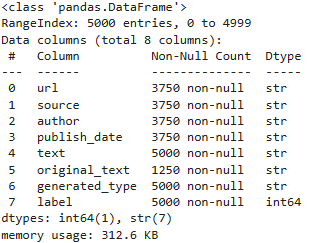
\includegraphics[width=0.5\textwidth]{images/chapter_03/img_15.png}
    \caption{Cấu trúc dữ liệu của hệ thống}
    \label{fig:nlp}
\end{figure}

\vspace{\baselineskip}
\noindent
\begin{table}[H]
    \centering
    \begin{tabular}{>{\bfseries}p{3.0cm}p{2.2cm}p{8.2cm}}
        \toprule
        Trường & Loại & Ý nghĩa \\
        \midrule
        \texttt{url} & \texttt{Metadata} & Nguồn URL của các bài báo \\
        \texttt{source} & \texttt{Metadata} & Tên miền của các bài báo. \\
        \texttt{author} & \texttt{Metadata} & Tên tác giả của bài báo. \\
        \texttt{publish\_date} & \texttt{Metadata} & Ngày xuất bản bài báo. \\
        \texttt{text} & \texttt{Đặc trưng đầu vào} & Nội dung văn bản được sử dụng cho quá trình huấn luyện và dự đoán. \\
        \texttt{original\_text} & \texttt{Dữ liệu tham chiếu} & Văn bản gốc trước khi được mô hình ngôn ngữ viết lại. \\
        \texttt{generated\_type} & \texttt{Metadata} & Phương tháp tạo ra bài báo. \\
        \texttt{label} & \texttt{Nhãn} & Nhãn phân loại, biểu thị văn bản Human hoặc AI. \\
        \bottomrule
    \end{tabular}
    \caption{Mô tả các trường trong tập dữ liệu}
    \label{tab:data_structure}
\end{table}

\noindent
Như vậy, bộ dữ liệu được tổ chức với trường thông tin được sử dụng để lưu trữ nội dung văn bản, nhãn phân loại và các thông tin liên quan đến nguồn dữ liệu. 
Ngoài ra, \texttt{text} là nội dung bài báo và \texttt{label} là thành phần chính để phục vụ cho quá trình mô hình học và dự đoán, còn các trường còn lại được
sử dụng cho mục đích phân tích và khai thác sâu vào dữ liệu.

\subsection{Phân bố dữ liệu}
Như ta đã thấy ở Hình 15, dữ liệu là tổng cộng gồm có 5000 mẫu. Trong đó, cột \texttt{label} được chia thành hai lớp có số lượng mẫu bằng nhau, đó là lớp AI và Human có
số lượng mẫu đều là 2500 mẫu.

\begin{figure}[H]
    \centering
    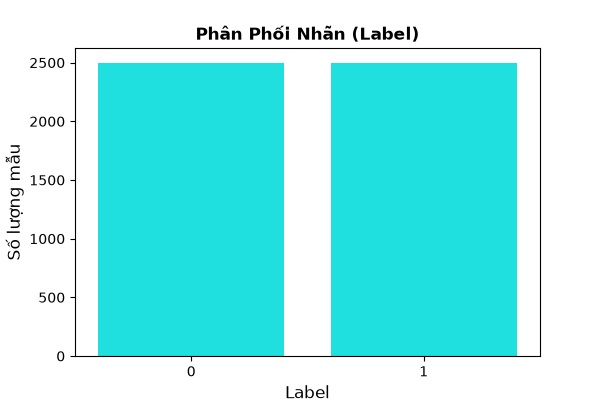
\includegraphics[width=0.8\textwidth]{images/chapter_03/img_16.png}
    \caption{Phân bố nhãn \texttt{label}}
    \label{fig:nlp}
\end{figure}

\noindent
Ngoài ra, trường \texttt{generated\_type} cũng đã phân bố đều, với ba thành phần đó là Human, Generated (bài báo do AI sinh ra hoàn toàn từ đầu), Rewritten (bài báo do AI viết
lại từ bài báo của con người, có nguồn rõ ràng). Dữ liệu cũng được tổ chức, phân bố đều với Human chiếm tới 2500 mẫu và hai thành phần còn lại, mỗi phần tương ứng 1250 mẫu.

\begin{figure}[H]
    \centering
    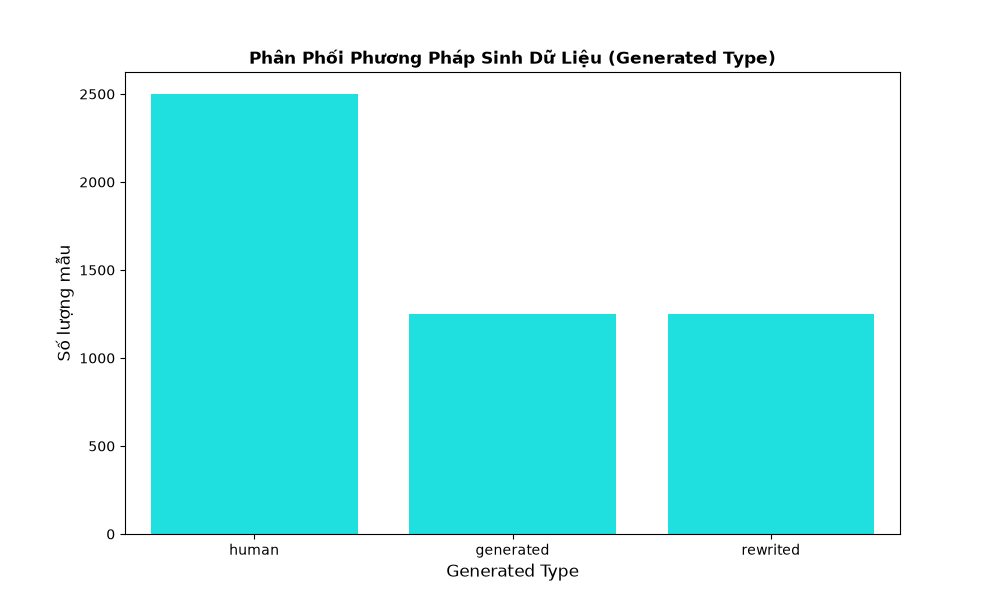
\includegraphics[width=0.9\textwidth]{images/chapter_03/img_17.png}
    \caption{Phân bố phương pháp tạo sinh dữ liệu}
    \label{fig:nlp}
\end{figure}

\noindent
Bên cạnh sự phân bố nhãn và phương pháp sinh dữ liệu, độ dài văn bẳn cũng là một yếu tố, đặc điểm cần đáng được xem xét trong quá trình phân tích toàn bộ dữ liệu. Sự khác biệt độ dài giữa
các nhóm văn bản có thể thể phản ánh những đặc điểm khác nhau trong quá trình biên soạn và tạo nội dung, đồng thời đánh giá được mức độ tương đồng về mặt độ dài giữa dữ liệu AI và Human.

\begin{figure}[H]
    \centering
    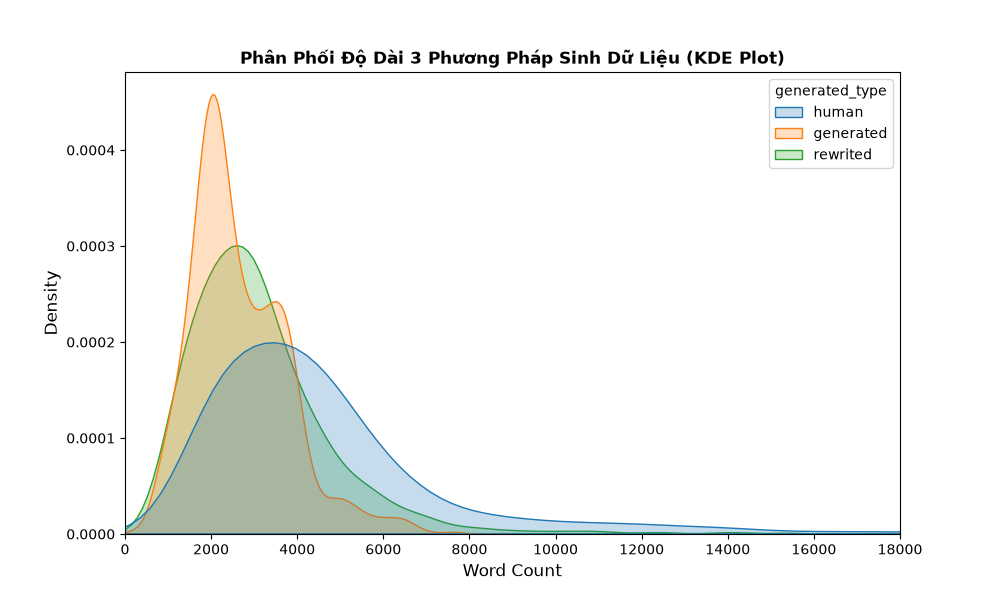
\includegraphics[width=1.0\textwidth]{images/chapter_03/img_18.png}
    \caption{Phân bố độ dài của các phương pháp tạo sinh dữ liệu}
    \label{fig:nlp}
\end{figure}

\noindent
Biểu đồ ước lượng mật độ nhân (Kernel Density Estimate - KDE) là một loại biểu đồ được sử dụng để trực quan hóa sự phân phối của một tập dữ liệu liên tục. Ở hình 18 trên, biểu đồ thể hiện mật dộ của phân
phối số lượng từ dựa trên ba phương pháp sinh dữ liệu. 

\vspace{\baselineskip}
\noindent
Ta có thể thấy nhóm sử dụng AI để tự sinh dữ liệu từ đầu (Generated) có mật độ cao nhất, nằm trong khoảng 2.000 - 3.500 từ và một số ít tập trung vào khoảng gần 4.000 - 4.500 từ ở mỗi bài. Điều này dữ liệu AI sinh văn bản
từ đầu trong đồ án có xu hướng tuân theo một khuôn mẫu về độ dài, ít biến động và phần lớn độ dài của văn bản khá là tương đồng.

\vspace{\baselineskip}
\noindent
Ngoài ra, nhóm Human có mật độ phân bố trải rộng rõ rệt hơn so với hai nhóm còn lại, khoảng 3.500 - 4.500 từ mỗi bài. Ở phía bên phải còn tồn tại rất nhiều văn bản trải rộng, tức là còn tồn tại nhiều văn bản có độ dài lớn
hơn so với mặt bằng chung. Điều này phản ánh tính đa dạng của nhóm Human khi xây dựng các nội dung bài báo so với hai nhóm còn lại. 

\vspace{\baselineskip}
\noindent
Tuy vậy, mật độ phân phối độ dài của ba nhóm có một phần chồng lấn, tập trung từ 2.000 - 4.000 từ khá nhiều. Cho thấy được độ dài cũng chưa phải là một đặc trưng đủ mạnh để mô hình đưa ra quyết định, còn phải phụ thuộc thêm ngữ nghĩa,
cấu trúc câu và từ vựng của từng loại bài báo.


\section{Tiền xử lý dữ liệu}
\subsection{Làm sạch và chuẩn hóa văn bản}
Sau khi đã phân tích, tìm hiểu cấu trúc, sự phân bố dữ liệu thì ta sẽ thực hiện quát trình làm sạch dữ liệu. Trong đồ án, quá trình làm sạch dữ liệu gồm ba bước: loại bỏ HTML, URL và loại bỏ khoảng trắng đầu và cuối của chuỗi, lý do là vì các mã code hay đường dẫn thì nó
không phản ánh cách viết của người hay AI và khoảng trắng chỉ làm tốn tài nguyên xử lý mà không mang lại giá trị ngữ nghĩa.

\begin{lstlisting}[style=pythoncode]
def clean_text(text):
    text = BeautifulSoup(text, 'html.parser').get_text()
    text = re.sub(r'http\S+|www\S+', '', text)
    text = re.sub(r'\s+', ' ', text).strip()
    return text
\end{lstlisting}

\captionof{listing}{Hàm làm sạch dữ liệu}

\begin{figure}[H]
    \centering
    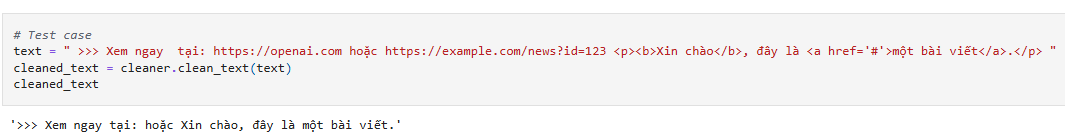
\includegraphics[width=1.0\textwidth]{images/chapter_03/img_19.png}
    \caption{Đoạn văn bản sau khi đã làm sạch}
    \label{fig:nlp}
\end{figure}

\noindent
Tuy nhiên vẫn có một điều cần làm rõ là trong đồ án phân loại văn bản AI này thì vẫn giữ nguyên dấu câu, chữ hoa, chữ thường, định dạng từ và các biểu cảm của văn bản gốc. Lý do là vì các thành phần đó là tín hiệu cực mạnh để phân biệt văn bản do người viết hay do AI tạo ra, các
thành phần đó cung cấp thông tin về phong cách viết, cấu trúc câu và cách sử dụng ngôn ngữ cho mô hình phân loại. Nhưng em vẫn không thể khẳng định đây là những đặc điểm chính xác luôn có khả năng phân biệt giữa con người viết hay do AI tạo ra. Bởi vì một tác giả họ có thể có khả 
năng viết một bài báo rất mạch lạc, tuân thủ nguyên tắc và sử dụng dấu câu một cách chính xác, trong khi các mô hình LLM hiện nay cũng có khả năng tạo ra văn bản giống như con người. Vì vậy, đồ án đã không loại bỏ những thành phần này mà giữ nguyên chúng để mô hình có thể tự học mức
độ đóng góp của từng đặc điểm dựa trên dữ liệu huấn luyện, thay vì áp đặt một đặc điểm nào đó chắc chắn là của Human hay là AI, tức là ví dụ như văn bản có nhiều dấu câu thì mình dự đoán đó là AI hay văn bản có lỗi chính tả là của Human thì các giả định này không phải lúc nào cũng đúng.

\subsection{Tokenization}
Sau bước làm sạch dữ liệu, bước tiếp theo là tokenization, tức là token hóa, nhằm chuyển đổi văn bản từ dạng chuỗi ký tự sang các đơn vị nhỏ hơn được gọi là token, token ở đây có thể là ký tự, thành phần của từ đó hay chính từ đó. Trong đồ án, em sử dụng bộ token hóa là của mô hình BamiBERT thông qua thư viện HuggingFace Transformer.

\vspace{\baselineskip}
\begin{lstlisting}[style=pythoncode]
from transformers import AutoTokenizer
tokenizer = AutoTokenizer.from_pretrained("Qualcomm-AI-Research/BamiBERT")
\end{lstlisting}

\captionof{listing}{Định nghĩa bộ token hóa BamiBERT}

\noindent
Bộ token hóa của mô hình BamiBERT sử dụng thuật toán Byte-level Byte Pair Encoding (BBPE), tức là thuật toán có khả năng tách một từ thành token dựa vào các tiêu chí nhất định dựa vào bộ từ vựng mà mô hình đã được huấn luyện, bao gồm từ phổ biến thì sẽ giữ nguyên cả từ (ví dụ: bánh mì $\rightarrow$ bánh\_mì), từ hiếm hoặc từ mới thì sẽ tách thành các thành 
phần con (subwords) và các từ hoàn toàn chưa biết thì sẽ được tách thành ký tự đơn.

\begin{lstlisting}[style=pythoncode]
MAX_LENGTH = 1024
it_ai_human_df['tokens'] = it_ai_human_df['cleaned_text'].apply(
    lambda x: tokenizer.tokenizer(
        x,
        max_length=MAX_LENGTH,
        truncation=True,
        padding='max_length',
        return_tensors='pt'
    )
)

# Extract input_ids + attention_mask
it_ai_human_df['input_ids'] = it_ai_human_df['tokens'].apply(lambda x: x['input_ids'][0].tolist())
it_ai_human_df['attention_mask'] = it_ai_human_df['tokens'].apply(lambda x: x['attention_mask'][0].tolist())
\end{lstlisting}

\captionof{listing}{Thực hiện token hóa văn bản}

\vspace{\baselineskip}
Quá trình tokenization sẽ được thực hiện ngay chính cột \texttt{cleaned\_text}, tức là cột chứa các văn bản sau khi đã làm sạch với độ dài tối đa mà bộ token hóa xử lý là 1024 token (\texttt{MAX\_LENGTH}). Nếu mà đoạn văn bản có độ dài vượt quá 1024 token thì sẽ thực hiện cắt đoạn ngay token thứ 1024 đó (truncation), còn các đoạn văn bản mà có độ dài nhỏ hơn 1024 token thì
sẽ chèn thêm các token \texttt{<PAD>} để cho đủ độ dài mà mô hình ban đầu giới hạn cho phép. Sau đó, các token sẽ được ánh xạ thành hai thành phần, đó là \texttt{input\_ids} và \texttt{attention\_mask}.

\vspace{\baselineskip}
\noindent
Trong đó, \texttt{input\_ids} là dãy số đại diện cho các token trong văn bản, ví dụ như các token sau: \texttt{["Sự", "xuất", "hiện", "của", "iPhone", "17e", ...]} thì sẽ ánh xạ
thành \texttt{[2470, 621, 447, 275, 4189, 1377, ...]}, mỗi con số thì sẽ tương ứng với một token trong bộ từ điển của tokenizer BamiBERT. \texttt{attention\_mask} sẽ cho mô hình BamiBERT biết token nào là token thật và token nào là padding, token padding ở đây chính là những token mà tokenizer sẽ chèn vào nếu độ dài của văn bản đó không đủ 1024 token, ví dụ như \texttt{input\_ids} 
gồm các ID của văn bản như sau:\texttt{[101, 2470, 621, 447, 275, 102, 0, 0, 0, ...]} thì \texttt{attention\_mask} sẽ ánh xạ thành \texttt{[1, 1, 1, 1, 1, 1, 0, 0, 0, ...]}. Trong đó 1 tương ứng với token thật, mô hình cần phải chú ý đến và 0 tức là token padding, mô hình sẽ bỏ qua. Hai thành phần đó đóng vai trò quan trọng cho việc phối hợp cùng nhau để cho mô hình học sâu được sử dụng
để huấn luyện có thể xử lý các văn bản có độ dài khác nhau sau khi được padding về cùng kích thước.

\section{Xây dựng và fine-tuning mô hình phân loại}
\subsection{Tạo group ID}
Bởi vì trong quá trình tạo dữ liệu AI-rewritten, em có sử dụng dữ liệu Human đã thu thập được làm văn bản gốc rồi sử dụng LLM để viết lại, nên là phải có một bước ghép các đoạn văn bản có \texttt{original\_text} (AI-rewritten) trùng với lại \texttt{text} (Human) để tránh bị lộ dữ liệu trong quá trình huấn luyện, ví dụ như nếu trong quá trình kiểm tra (test) mà xuất hiện một đoạn văn bản có \texttt{original\_text}
trùng với lại \texttt{text} của đoạn văn bản đó trong quá trình huấn luyện thì mô hình vô tình đã biết trước dữ liệu, điều này dẫn đến khả năng tổng quát hóa của mô hình kém đi.

\begin{figure}[H]
    \centering
    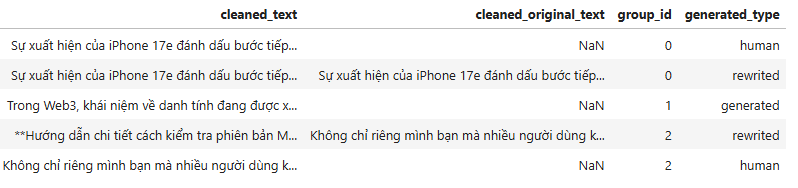
\includegraphics[width=1.0\textwidth]{images/chapter_03/img_20.png}
    \caption{Đoạn văn bản sau đã nhóm theo ID}
    \label{fig:nlp}
\end{figure}

\subsection{Chia tập dữ liệu}
Sau khi đã tạo \texttt{group\_id}, ta sẽ tiến hành chia tập dữ liệu thành ba phần: tập huấn luyện (train), tập xác thực (validation) và tập kiểm thử (test). Việc chia dữ liệu theo \texttt{group\_id} đảm bảo các văn bản có không bị trùng \texttt{original\_text} và \texttt{text} ở nhiều tập dữ liệu. Sau khi chia, dữ liệu 
gồm 3.502 mấu cho tập train, 766 cho tập validation và 732 cho tập test, tức là tỉ lệ xấp xỉ 70/15/15.

\begin{figure}[H]
    \centering
    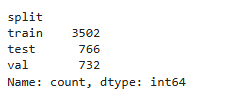
\includegraphics[width=0.4\textwidth]{images/chapter_03/img_21.png}
    \caption{Tỉ lệ tập dữ liệu sau khi chia}
    \label{fig:nlp}
\end{figure}

\subsection{Định nghĩa mô hình phân loại phù hợp với bài toán}

\begin{lstlisting}[style=pythoncode]
class AIContentModel(nn.Module):
    """
    BamiBert Encoder + Classification Head.
    """
    def __init__(self, model_name='Qualcomm-AI-Research/BamiBERT', num_classes=2, dropout=0.1):
        super().__init__()
        self.bert = AutoModel.from_pretrained(model_name)
        hidden_size = self.bert.config.hidden_size # 768 for base 
        self.dropout = nn.Dropout(dropout)
        self.classifier = nn.Linear(hidden_size, num_classes)

    def forward(self, input_ids, attention_mask):
        outputs = self.bert(input_ids=input_ids, attention_mask=attention_mask)

        # [CLS] token represents for first token
        cls_output = outputs.last_hidden_state[:, 0, :]
        x = self.dropout(cls_output)
        logits = self.classifier(x)

        return logits
\end{lstlisting}

\captionof{listing}{Định nghĩa mô hình phân loại}
Trong đồ án, em sẽ tự định nghĩa mô hình phân loại thành một class riêng, mô hình \texttt{AIContentModel}. Đây là mô hình được định nghĩa dựa trên mô hình nền BamiBERT và được thiết kế riêng
cho bài toán phân loại văn bản AI. Kích thước biểu diễn vector sẽ lấy từ mô hình BamiBERT thông qua \texttt{hidden\_size} với 768 chiều. Vector biễu diên của token \texttt{[CLS]} tại vị trí đầu tiên
của chuỗi văn bản được lấy từ \texttt{last\_hidden\_state}, vì đây là nơi mà mô hình BamiBERT lưu toàn bộ các vector biểu diễn của các token sau khi đã đi qua toàn bộ layer của quá trình Encoder.

\vspace{\baselineskip}
\noindent
Sau đó, vector này sẽ đi qua lớp Dropout, là một lớp có khả năng giảm hiện tượng quá khớp (overfitting) bằng cách tắt ngẫu nhiên một số neuron trong quá trình huấn luyện.

\begin{figure}[H]
    \centering
    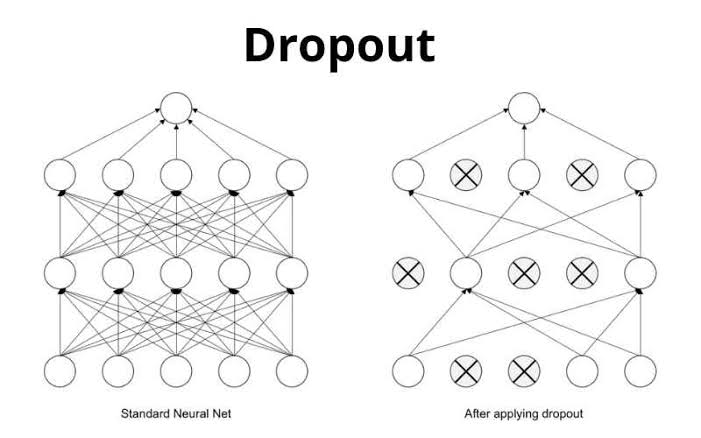
\includegraphics[width=0.7\textwidth]{images/chapter_03/img_22.jpg}
    \caption{Hiện tượng dropout trong mạng neuron}
    \label{fig:nlp}
\end{figure}

\vspace{\baselineskip}
\noindent
Cuối cùng, các vector đó sẽ được đưa vào lớp Classification Head để ánh xạ vector 768 chiều sang 2 chiều, 2 chiều ở đây sẽ mang giá trị là logit tương ứng với 2 lớp.

\subsection{Fine-tuning mô hình phân loại}
Sau khi đã xây dựng xong mô hình thì sẽ tiến hành quá trình fine-tuning mô hình trên tập dữ liệu đã được tiền xử lý. Quá trình này sẽ thực hiện tinh chỉnh các tham số mô hình
sao cho phù hợp với yêu cầu của bài toán đồ án.

\begin{lstlisting}[style=pythoncode]
criterion = nn.CrossEntropyLoss()
optimizer = AdamW(model.parameters(), lr=2e-5)
num_epochs = 3 
\end{lstlisting}

\captionof{listing}{Định nghĩa tham số mô hình}
Trong đó, \texttt{CrossEntropyLoss} được sử dụng để đo lường mức độ sai số giữa kết quả dự đoán của mô hình so với nhãn thực tế.

\begin{equation}
    \mathcal{L}_{\mathrm{CE}} = -\frac{1}{N} \sum_{i=1}^{N} \sum_{c=1}^{C} y_{i,c} \log\left(p_{i,c}\right)
\end{equation}

\captionof{listing}{Công thức CrossEntropy}

Trong đó:
\begin{itemize}
    \item $N$ là số lượng mẫu trong một batch.
    \item $C$ là số lượng lớp cần phân loại, trong đồ án này $C=2$, gồm lớp Human và AI.
    \item $y_{i,c}$ là giá trị nhãn thực tế của mẫu thứ $i$ đối với lớp $c$. Giá trị này bằng 1 nếu mẫu thuộc lớp $c$ và bằng 0 trong các trường hợp còn lại.
    \item $p_{i,c}$ là xác suất dự đoán mẫu thứ $i$ thuộc lớp $c$, được tính bằng hàm Softmax từ các giá trị logit do mô hình tạo ra.
    \item $\log$ là hàm logarithm tự nhiên. Giá trị Cross Entropy càng nhỏ thì kết quả dự đoán càng gần với nhãn thực tế.
\end{itemize}

\texttt{AdamW} là một thuật toán tối ưu với tỉ lệ học (\texttt{learning\_rate}). Thuật toán này sẽ cập nhật tham số dựa vào gradient trong quá trình lan truyền ngược.

Với gradient $g_t = \nabla_{\theta}\mathcal{L}_t$ tại bước huấn luyện thứ $t$, thuật toán AdamW thực hiện các bước tính toán moment như sau:

\begin{align}
    m_t &= \beta_1 m_{t-1} + (1-\beta_1)g_t, \\
    v_t &= \beta_2 v_{t-1} + (1-\beta_2)g_t^2, \\
    \hat{m}_t &= \frac{m_t}{1-\beta_1^t}, \qquad
    \hat{v}_t = \frac{v_t}{1-\beta_2^t}, \\
    \theta_{t+1} &= \theta_t - \alpha \left( \frac{\hat{m}_t}{\sqrt{\hat{v}_t} + \epsilon} + \lambda \theta_t \right).
\end{align}

\captionof{listing}{Thuật toán AdamW}

Trong đó:
\begin{itemize}
    \item $\theta_t$ là các tham số của mô hình tại bước huấn luyện thứ $t$; $\theta_{t+1}$ là các tham số sau khi được cập nhật.
    \item $g_t$ là gradient của hàm mất mát theo các tham số mô hình tại bước thứ $t$.
    \item $m_t$ là moment bậc nhất, dùng để lưu giá trị trung bình động của gradient và xác định hướng cập nhật.
    \item $v_t$ là moment bậc hai, dùng để lưu giá trị trung bình động của bình phương gradient và điều chỉnh kích thước bước cập nhật.
    \item $\beta_1$ và $\beta_2$ là các hệ số suy giảm của moment bậc nhất và bậc hai. Hai giá trị thường được sử dụng lần lượt là $0{,}9$ và $0{,}999$.
    \item $\hat{m}_t$ và $\hat{v}_t$ là các moment đã được hiệu chỉnh bias, giúp giảm ảnh hưởng của việc khởi tạo $m_0$ và $v_0$ bằng 0.
    \item $\alpha$ là learning rate, quy định độ lớn của bước cập nhật tham số. Trong đoạn mã trên, $\alpha=2\times10^{-5}$.
    \item $\lambda$ là hệ số weight decay, giúp hạn chế hiện tượng overfitting bằng cách điều chỉnh tham số về gần 0.
    \item $\epsilon$ là một giá trị dương rất nhỏ, giúp tránh phép chia cho 0 khi tính toán.
\end{itemize}
Tiếp theo là ta sẽ tiến hành huấn luyện mô hình, quá trình huấn luyện được thể hiện qua đoạn code sau:

\begin{lstlisting}[style=pythoncode]
def train_epoch(model, loader, optimizer, criterion, device):
    model.train()
    total_loss = 0
    correct = 0
    total = 0

    progress_bar = tqdm(loader, desc='Training', leave=False, position=1)

    for batch in progress_bar:
        input_ids = batch['input_ids'].to(device)
        attention_mask = batch['attention_mask'].to(device)
        labels = batch['labels'].to(device)

        optimizer.zero_grad()
        logits = model(input_ids, attention_mask)
        loss = criterion(logits, labels)
        loss.backward()
        optimizer.step()

        total_loss += loss.item()
        preds = torch.argmax(logits, dim=1)
        correct += (preds == labels).sum().item()
        total += labels.size(0)

        progress_bar.set_postfix({
            'Loss': f'{loss.item():.4f}',
            'Accuracy': f'{correct/total:.4f}'
        })

    return total_loss / len(loader), correct / total
\end{lstlisting}

\captionof{listing}{Huấn luyện mô hình}
Sau khi đã thiết lập tham số cho quá trình fine-tuning. Mô hình sẽ bắt đầu huấn luyện thông qua hàm \texttt{train\_epoch}. Đầu tiên, ta sẽ chuyển mô hình sang trạng thái huấn luyện \texttt{model.train()} rồi sau đó tiến hành
huấn luyện theo batch. Mỗi batch ta sẽ lọc ra ba thành phần để phục vụ training, đó là \texttt{input\_ids} biểu diễn các token của văn bản dưới dạng chuỗi số, \texttt{attention\_mask} cho biết token nào là token thật và 
token nào là padding và \texttt{labels} chính là nhãn mục tiêu tương ứng với hai lớp AI và Human. Đối với mỗi batch, gradient của những lần được cập nhật trước sẽ xóa bằng \texttt{zero\_grad()} trước khi thực hiện quá trình lan
truyên xuôi. Dữ liệu sau đó sẽ được đưa vào mô hình để tạo ra các vector biểu diễn rồi sau đó sẽ ánh xạ thành các giá trị logit và gán vào biến \texttt{logits}. Tiếp theo, giá trị logit đó sẽ kết hợp với nhãn thực thế (labels) để
tính sai số rồi bắt đầu lan truyền ngược \texttt{loss.backward()} nhằm tính gradient của hàm mất mát đối với các tham số của mô hình. Sau đó việc cập nhật trọng số sẽ được thực hiện thông qua \texttt{optimizer.step()}.

\vspace{\baselineskip}
\noindent
Bên cạnh việc cập nhật trọng số thì em sẽ lấy kết quả dự đoán của từng batch để tính toán độ chính xác. Lớp có giá trị lớn nhất sẽ được lấy thông qua hàm \texttt{argmax} rồi sẽ cập nhật thông qua biến \texttt{correct}.

\begin{lstlisting}[style=pythoncode]
def evaluate(model, loader, criterion, device):
    model.eval()
    total_loss = 0
    correct = 0
    total = 0

    with torch.no_grad():
        progress_bar = tqdm(loader, desc='Validation', leave=False, position=1)

        for batch in progress_bar:
            input_ids = batch['input_ids'].to(device)
            attention_mask = batch['attention_mask'].to(device)
            labels = batch['labels'].to(device)

            logits = model(input_ids, attention_mask)
            loss = criterion(logits, labels)

            total_loss += loss.item()
            preds = torch.argmax(logits, dim=1)
            correct += (preds == labels).sum().item()
            total += labels.size(0)

            progress_bar.set_postfix({
                'Loss': f'{loss.item():.4f}',
                'Accuracy': f'{correct/total:.4f}'
            })
            
    return total_loss / len(loader), correct / total
\end{lstlisting}
\captionof{listing}{Đánh giá mô hình}
Bên cạnh trong quá trình huấn luyện, ta cũng phải đánh giá dựa trên tập \texttt{validation} để biết được trong quá trình huấn luyện độ chính xác của mô hình tới đâu. Đầu
tiên, ta sẽ chuyển mô hình sang chế độ đánh giá (\texttt{model.eval()}), trạng thái này sẽ tắt lớp Dropout để phục vụ cho quá trình đánh giá. Về cơ bản hàm này chỉ khác hàm
\texttt{train\_epoch} là hàm này chỉ tập trung vào việc tính sai số (loss) kết hợp với độ chính xác (accuracy) trên tập \texttt{validation}.

\begin{lstlisting}[style=pythoncode]
for epoch in progress_bar:
    train_loss, train_acc = trainer.train_epoch(model, train_loader, optimizer, criterion, device)
    val_loss, val_acc = trainer.evaluate(model, val_loader, criterion, device)

    history['train_loss'].append(train_loss)
    history['train_acc'].append(train_acc)
    history['val_loss'].append(val_loss)
    history['val_acc'].append(val_acc)

    print(f'Epoch {epoch + 1} / {num_epochs}')
    print(f'Train | Loss: {train_loss:.4f} - Accuracy: {train_acc:.4f}')
    print(f'Valid | Loss: {val_loss:.4f} - Accuracy: {val_acc:.4f}')

    if val_acc > best_val_acc:
        best_val_acc = val_acc
        torch.save({
            'epoch': epoch,
            'model_state_dict': model.state_dict(),
            'optimizer_state_dict': optimizer.state_dict(),
            'best_val_acc': best_val_acc,
            }, checkpoint_path)
        print(f'Save new best model (val_acc = {val_acc:.4f})')
\end{lstlisting}
\captionof{listing}{Vòng lặp fine-tuning}
Trong mỗi epoch, các giá trị \texttt{loss} và \text{acc} sẽ được tính thông qua hai hàm, \texttt{train\_epoch} và \texttt{evaluate}. Sau đó nếu độ
chính xác của \texttt{val} mà lớn hơn so với \texttt{best\_val\_acc} thì sẽ tiến hành lưu trạng thái của mô hình lại (checkpoint), checkpoint này bao gồm
epoch hiện tại, trạng thái của mô hình, tức là trọng số của mô hình (\texttt{model\_state\_dict}) và trọng số của optimizer (\texttt{optimizer\_state\_dict}).
Việc lưu lại checkpoint giúp giữ lại trạng thái tốt nhất của model thay vì sử dụng trọng số ở epoch cuối cùng.

\vspace{\baselineskip}
\noindent
Toàn bộ quá trình fine-tune mô hình có thể được thể hiện thông qua sơ đồ sau:

\begin{figure}[H]
    \centering
    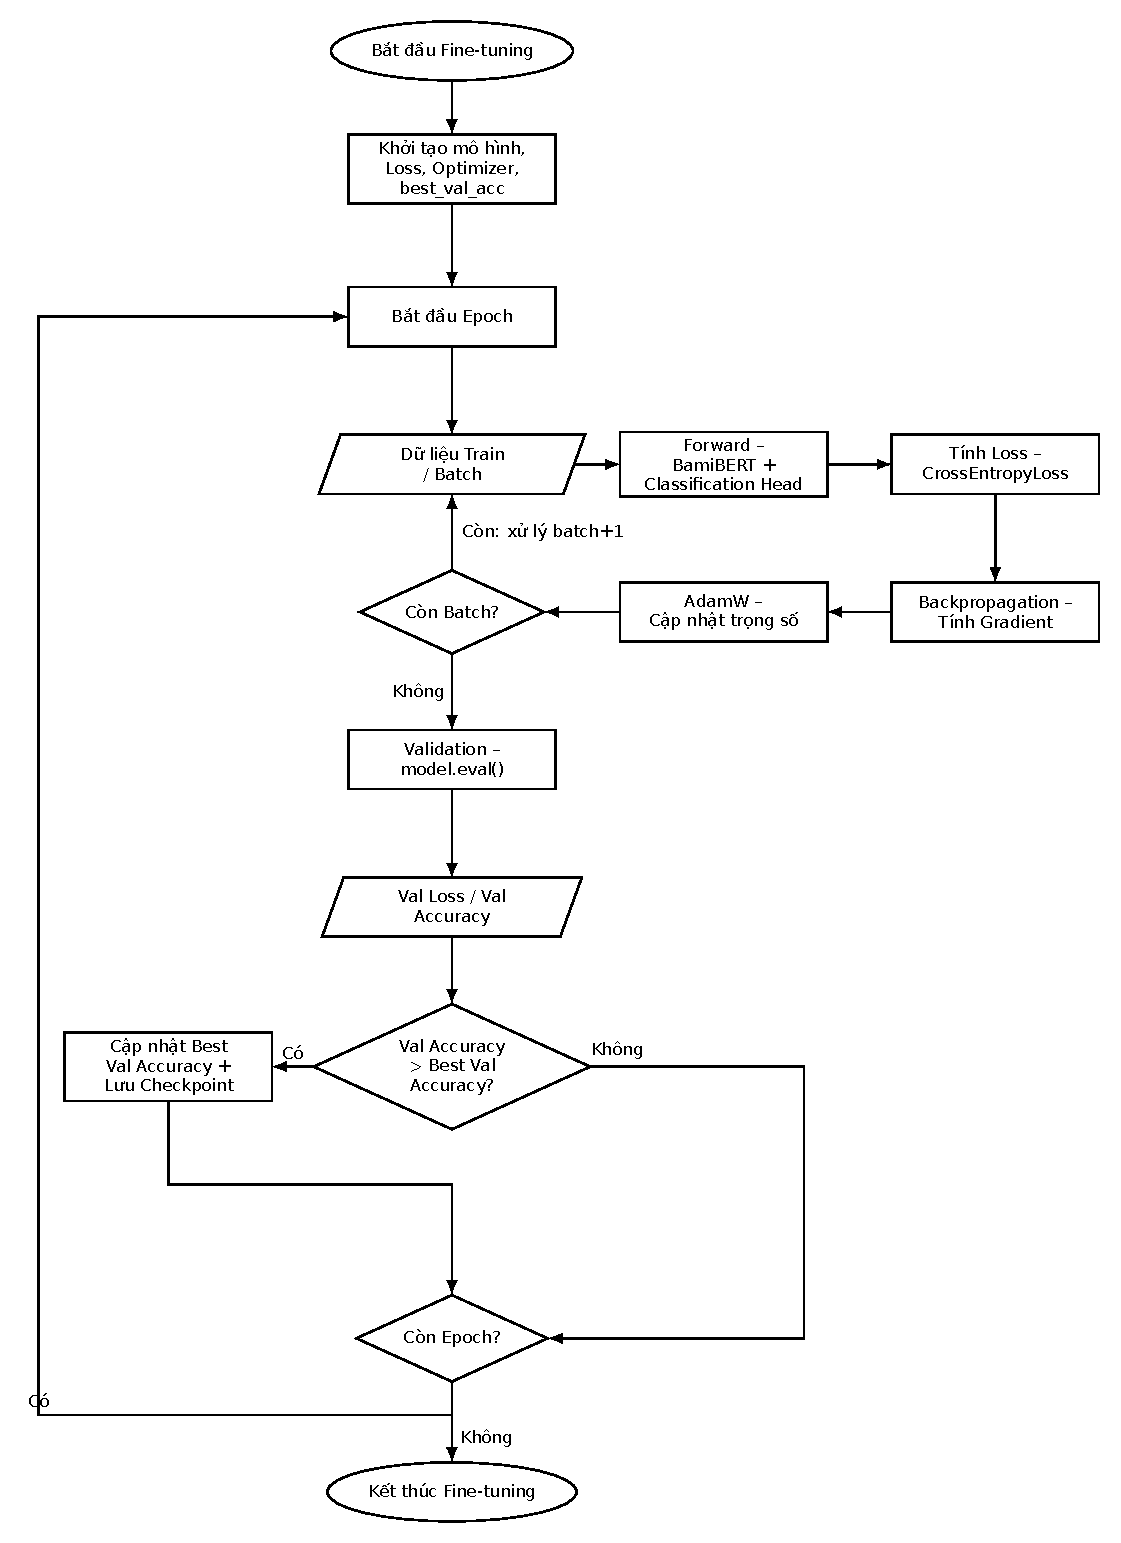
\includegraphics[width=1.1\textwidth]{figures/chapter_03/fine_tune_workflow.pdf}
    \caption{Quá trình fine-tuning}
    \label{fig:fine_tune_workflow}
\end{figure}

\noindent
Qua quá trình fine-tune, mô hình có trọng số tốt nhất được lưu tại \texttt{best\_model.pt} nằm ở epoch số 3 với \texttt{val\_acc = 0.9604}:

\begin{figure}[H]
    \centering
    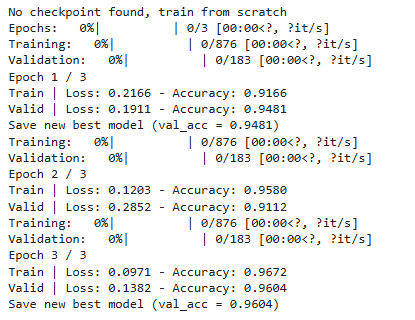
\includegraphics[width=0.5\textwidth]{images/chapter_03/img_24.png}
    \caption{Điểm của mô hình huấn luyện qua các epoch}
    \label{fig:nlp}
\end{figure}

\section{Xây dựng chức năng giải thích}
\subsection{Tổng quan quy trình giải thích}
Sau khi mô hình đã đưa ra dự đoán, hệ thống còn kết hợp chức năng giải thích, giải thích ở đây là gồm hai loại, đó là giải thích mức độ đóng góp của từng token dựa trên kết quả dự đoạn và giải
thích dựa trên các chỉ số định lượng, các token đó bằng ngôn ngữ tự nhiên thông qua mô hình LLM.

\vspace{\baselineskip}
\noindent
Quy trình cụ thể như sau: Văn bản đầu vào sẽ được chia thành hai luồng, một luồng là sẽ đưa vào mô hình BamiBERT để xử lý đưa ra kết quả dự đoán (1) và luồng còn lại sẽ tính đặc trưng thống kê (2). Luồng (1) sau khi đã 
đưa ra kết quả dự đoán thì sẽ sử dụng thuật toán Integrated Gradients (XAI) để bắt đầu tính attribution scores đối với lại từng token, sau đó nếu người dùng yêu cầu giải thích bằng LLM thì sẽ trích ra các top tokens có score
cao nhất còn không thì sẽ hiển thị kết quả dưới dạng highlight. Luồng (2) sẽ thực hiện tính các đặc trưng thống kê, các đặc trưng ở đây cụ thể là mật độ dấu câu, độ dài câu, số câu,\dots làm các giá trị định lượng cho LLM. Sau
đó kết quả từ hai luồng sẽ được tổng hợp lại và sẽ đưa vào LLM (Gemini) để sinh ra giải thích. 

\vspace{\baselineskip}
\noindent
Luồng hoạt động được thể hiện bằng sơ đồ sau:

\begin{figure}[H]
    \centering
    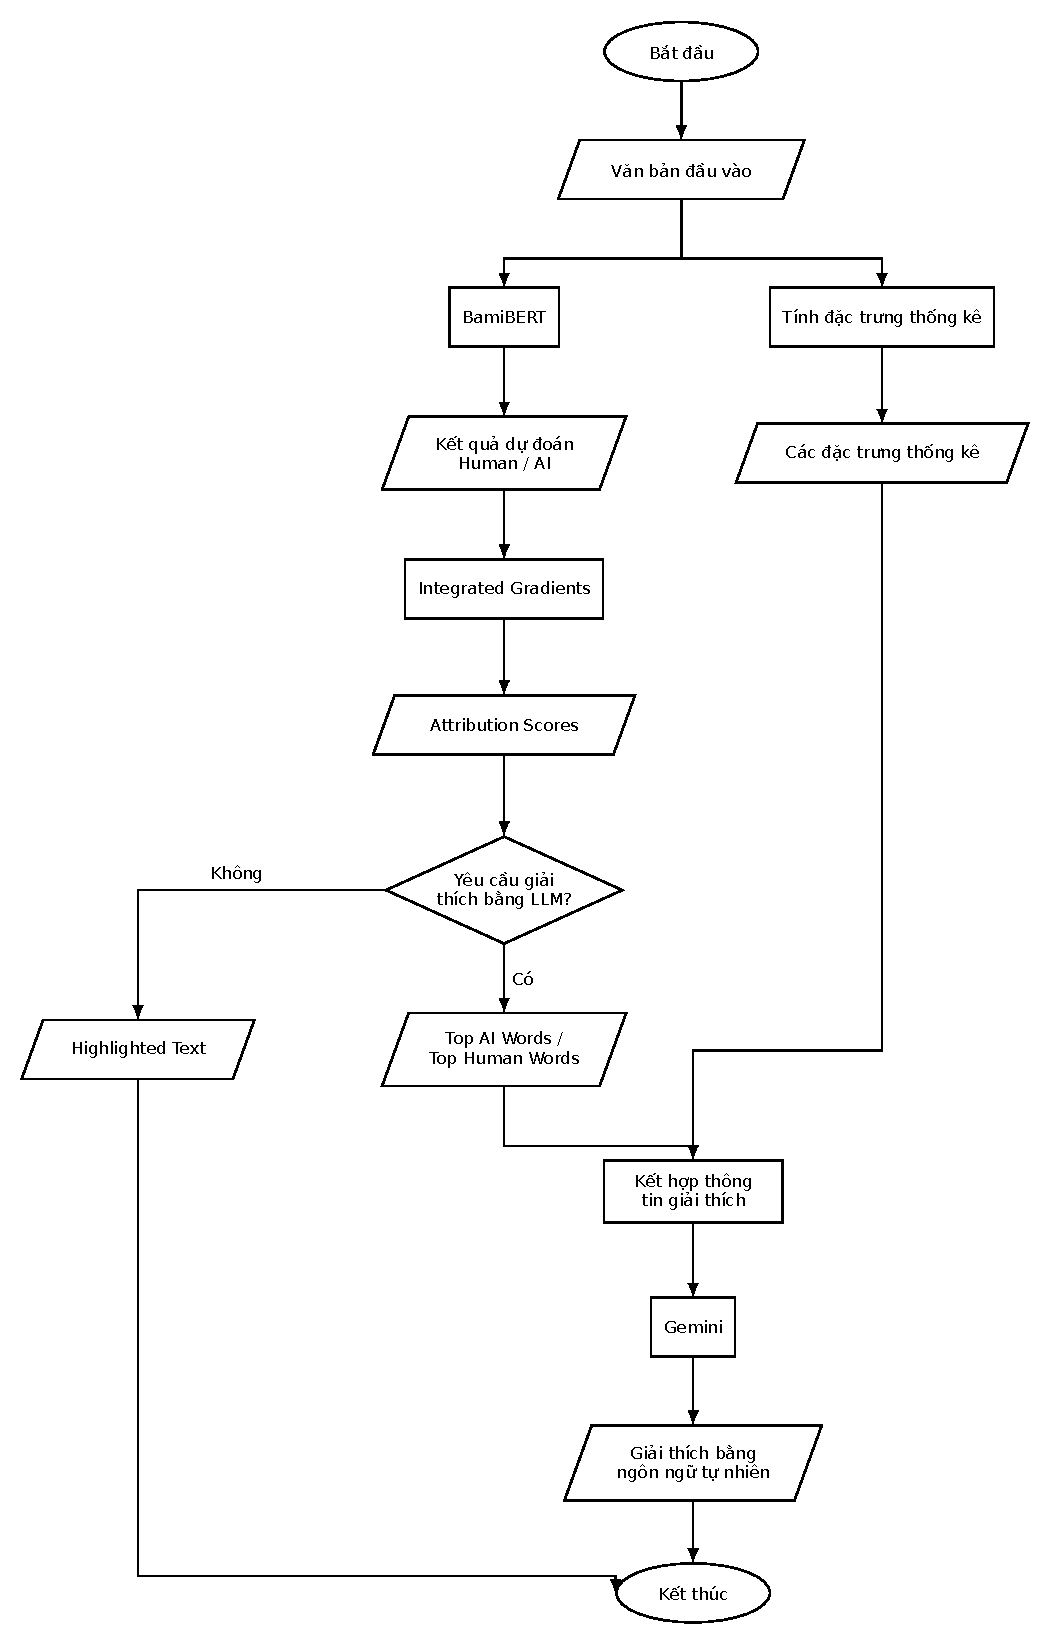
\includegraphics[width=1.0\textwidth]{figures/chapter_03/explain_workflow.pdf}
    \caption{Quá trình đưa ra giải thích}
    \label{fig:fine_tune_workflow}
\end{figure}

\subsection{Tính toán mức độ đóng góp bằng Integrated Gradients}
Trong hệ thống, mức độ đóng góp của từng token sẽ được tính bằng thuật toán Integrated Gradients, thông qua lớp \texttt{LayerIntegratedGradients} của module \texttt{captum}.

\begin{lstlisting}[style=pythoncode]
self.lig = LayerIntegratedGradients(self._forward_func, self.model.bert.embeddings)

def _forward_func(self, input_ids, attention_mask):
    logits = self.model(input_ids, attention_mask)
    return logits
\end{lstlisting}
\captionof{listing}{Khởi tạo \texttt{LayerIntegratedGradients}}

Lớp \texttt{LayerIntegratedGradients} sẽ tính toán mức độ attribution của từng token đầu vào. Trong đó, lớp embedding của mô hình BamiBERT được chọn làm lớp mục tiêu để tính attribution, vì 
lớp này là lớp biểu diễn vector của từng token, do đó attribution sẽ được tính tại lớp này và quy về từng token rồi ánh xạ ngược lại từng từ/cụm từ trong văn bản. Hàm lan truyển sẽ nhận \texttt{input\_ids} và
\texttt{attention\_mask} làm đầu vào để tính giá trị logits, làm đầu ra tương ứng cho các lớp cần phân loại.

\begin{lstlisting}[style=pythoncode]
encoding = self.tokenizer(
        text, max_length=self.max_length, truncation=True,
        padding='max_length', return_tensors='pt',
        return_offsets_mapping=True # return position of each token
        )
input_ids = encoding['input_ids'].to(self.device)
attention_mask = encoding['attention_mask'].to(self.device)
offsets = encoding['offset_mapping'][0].tolist()  # [(start,end), ...] from original text

baseline_ids = torch.full_like(input_ids, self.tokenizer.pad_token_id)
\end{lstlisting}
\captionof{listing}{Chuẩn bị đầu vào và baseline cho quá trình tính attribution}

Trước khi tính attribution thì văn bản đầu vào sẽ được chuyển đổi thành \texttt{input\_ids} và \texttt{attention\_mask} thông qua tokenizer của BamiBERT. Ngoài ra hệ thống còn lưu lại vị trí
của từng token trên văn bản gốc thông qua \texttt{offset\_mapping}, ví dụ như chuỗi sau: "Tôi thích AI" sẽ được ánh xạ thành các chuỗi chỉ số "01234...." thì token "Tôi" sẽ được ánh xạ thành (0, 2). Việc
lưu lại vị trí nhằm hỗ trợ cho bước quy đổi giá trị attribution về từ hoặc cụm từ sau này. \texttt{baseline\_ids} đơn giản là làm đầu vào tham chiếu, tức là tạo một chuỗi có cùng kích thước với \texttt{input\_ids},
trong đó các token được thay bằng token \texttt{<PAD>} làm điểm xuất phát để IG đánh giá mức độ thay đổi khi chuyển từ baseline sang văn bản thực tế. Từ sự thay đổi đó, mức độ đóng góp của từng token qua kết quả dự
đoán được xác định.

\begin{lstlisting}[style=pythoncode]
attributions, delta = self.lig.attribute(
        inputs=input_ids, baselines=baseline_ids,
        additional_forward_args=(attention_mask,),
        target=target_label, return_convergence_delta=True, n_steps=n_steps
    )
\end{lstlisting}
\captionof{listing}{Thực hiện tính attribution}
Sau bước chuẩn bị đầu vào và baseline, attribution sẽ được tính thông qua hàm \texttt{attribute} của lớp \texttt{LayerIntegratedGradients} riêng cho lớp mục tiêu \texttt{target\_label}. Đồng thời còn để biết từ baseline đến
văn bản thật thì output của mô hình đã thay đổi bao nhiêu thì phải thông qua tham số định nghĩa số bước nội suy (\texttt{n\_steps}). Bên cạnh đó, tham số \texttt{return\_convergence\_delta} được sử dụng để đánh giá mức độ hội tụ
hay là độ chính xác của thuật toán IG, tức là giá trị này sẽ tính được sai số lệch giữa tổng attribution tính được so với mức thay đổi đầu ra thực tế giữa mô hình đầu vào so với baseline.

\subsection{Xử lý và tổng hợp Attribution}
Sau khi đã có attribution, giá trị của nó vẫn được biểu diễn theo vector embedding nhiều chiều, cụ thể là 768 chiều. Do đó, ta cần một bước để tổng hợp các giá trị attribution trên toàn bộ chiều của vector embedding thành một giá trị 
đại diện cho mức độ đóng góp của từng token.

\begin{lstlisting}[style=pythoncode]
attributions = attributions.sum(dim=-1).squeeze(0)
attributions = attributions / (torch.norm(attributions) + 1e-10) # keep in stable range
syllable_scores = attributions.cpu().detach().numpy()
\end{lstlisting}
\captionof{listing}{Tổng hợp và chuẩn hóa giá trị attribution}

Ở đây, ta sẽ tính tổng hợp bằng cách tính tổng toàn bộ các attribution trên vector nhiều chiều thống qua \texttt{attribution.sum(dim=-1)}, sau đó ta sẽ chuẩn hóa giá trị vừa tính được về cùng một thang đo để thuận tiện cho việc so sánh và
trực quan hóa.

\begin{lstlisting}[style=pythoncode]
attributions = attributions.sum(dim=-1).squeeze(0)
attributions = attributions / (torch.norm(attributions) + 1e-10) # keep in stable range
syllable_scores = attributions.cpu().detach().numpy()
\end{lstlisting}
\captionof{listing}{Tổng hợp và chuẩn hóa giá trị attribution}

Sau khi đã chuẩn hóa xong, các attribution lúc này vẫn là một giá trị của từng token nên ta phải thực hiện bước ánh xạ sang attribution của từng từ hay cụm từ.
\begin{lstlisting}[style=pythoncode]
from underthesea import word_tokenize as vn_word_tokenize

    vn_words = vn_word_tokenize(text)  # for example: ['Samsung', 'đang', 'gặp', 'khó khăn', ...]

# Step 3: Map for each compound nouns -> positional range from original text
word_spans = []
cursor = 0
for w in vn_words:
    start = text.find(w, cursor)
    if start == -1: # unnecessary, defensive programming
            continue
        end = start + len(w)
        word_spans.append((w, start, end))
        cursor = end

    # Step 4: Combine attribution of syllable-tokens to fall in range of each compound nouns
    word_results = []
    for word, w_start, w_end in word_spans:
        scores_in_span = [
            syllable_scores[i] for i, (s, e) in enumerate(offsets)
            if s < w_end and e > w_start and not (s == 0 and e == 0)  # drop special tokens
        ]
        if scores_in_span:
            word_results.append((word, float(np.mean(scores_in_span))))
\end{lstlisting}
\captionof{listing}{Ánh xạ giá trị token sang từ/cụm từ}
Ở đây, ta sẽ sử dụng hàm \texttt{word\_tokenize} của module \texttt{underthesea} để tách chuỗi văn bản thành các token tiếng Việt tương ứng, từ đơn
tách thành từ đơn cũng như từ ghép tách thành từ ghép, sau đó thực hiện gom attribution của các token có phần ký tự giao với từ hay cụm từ đang xét 
(\texttt{syllable\_scores[i] for i, (s, e) in enumerate(offsets)}). Nếu như gặp từ ghép thì ta sẽ tính trung bình các attribution của các token trong từ đó.

\subsection{Sinh giải thích bằng LLM}
Bênh cạnh khả năng giải thích dựa trên attribution score của từng từ thì hệ thống còn xây dựng thêm chức năng giải thích bằng ngôn ngữ tự nhiên. Đầu tiên, để cho lời
nhắc (prompt) mà sát với các kết quả mà hệ thống đưa ra thì ta cần phải tính thêm các giá trị định lượng và lọc ra các từ, cụm từ mà có attribution score cao để đưa vào 
mô hình LLM giải thích.

\begin{lstlisting}[style=pythoncode]
def compute_signals(cleaned_text, tokens, scores, top_k = 8):
    paired = sorted(zip(tokens, scores), key=lambda x: abs(x[1]), reverse=True)
    top_ai_words = [w for w, s in paired if s > 0][:top_k]
    top_human_words = [w for w, s in paired if s < 0][:top_k]

    sentences = [s.strip() for s in re.split(r'[.!?]', cleaned_text) if s.strip()]
    sentence_lengths = [len(s.split()) for s in sentences]
    punct_count = len(re.findall(r'[^\w\sÀ-ỹ]', cleaned_text))

    return {
        'top_ai_words': top_ai_words,
        'top_human_words': top_human_words,
        'sentence_count': len(sentences),
        'avg_sentence_length': sum(sentence_lengths) / max(len(sentence_lengths), 1),
        'sentence_length_std': statistics.pstdev(sentence_lengths) if len(sentence_lengths) > 1 else 0.0,
        'punctuation_density': punct_count / max(len(cleaned_text), 1)
    }
\end{lstlisting}
\captionof{listing}{Lọc các token có attribution lớn nhất và tính các giá trị định lượng}

\begin{table}[H]
\centering
\caption{Ý nghĩa các giá trị được tính trong quá trình sinh giải thích bằng LLM}
\label{tab:attribution-signals}
\begin{tabular}{|p{0.32\textwidth}|p{0.58\textwidth}|}
\hline
\textbf{Giá trị} & \textbf{Ý nghĩa} \\
\hline
\texttt{top\_ai\_words} & Các từ/cụm từ có mức độ đóng góp mạnh theo hướng nhãn AI \\
\hline
\texttt{top\_human\_words} & Các từ/cụm từ có mức độ đóng góp mạnh theo hướng nhãn Human \\
\hline
\texttt{sentence\_count} & Số lượng câu trong văn bản, phản ánh quy mô cấu trúc câu của văn bản \\
\hline
\texttt{avg\_sentence\_length} & Độ dài câu trung bình, cho biết một văn bản đó có xu hướng câu ngắn hay dài \\
\hline
\texttt{sentence\_length\_std} & Độ lệch chuẩn của câu, cho biết mức độ biến thiên của câu trong văn bản, tức là các câu trong văn bản có độ dài đồng đều hay không \\
\hline
\texttt{punctuation\_density} & Mật độ dấu câu, phản ánh mức độ dấu câu hay kí tự đặc biệt của văn bản \\
\hline
\end{tabular}
\end{table}

\section{Xây dựng backend}
\subsection{Mô hình thực thể kết hợp (ERD)}

\begin{figure}[H]
    \centering
    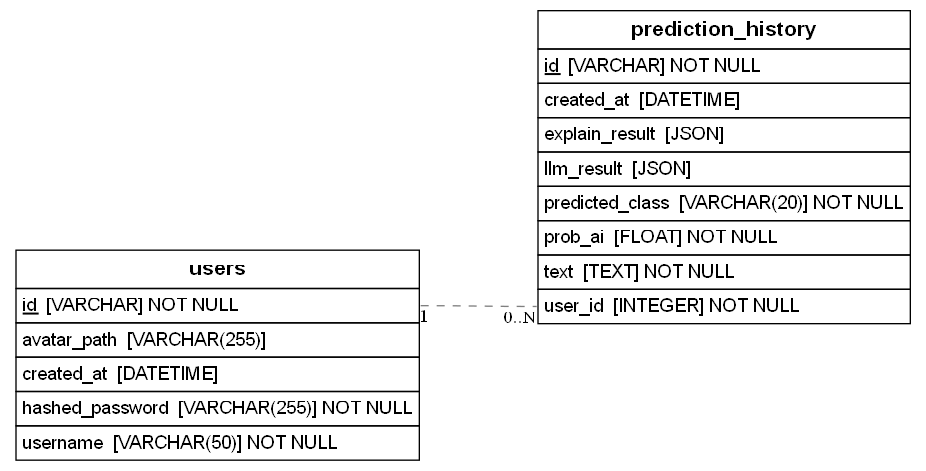
\includegraphics[width=0.8\textwidth]{images/chapter_03/img_25.png}
    \caption{Lược đồ trực quan hóa CSDL}
    \label{fig:fine_tune_workflow}
\end{figure}

\subsection{Thiết kế chi tiết các bảng}
\subsubsection{Bảng user}
Bảng này lưu trữ thông tin cho từng tài khoản người dùng.

\begin{table}[H]
\centering
\caption{Cấu trúc bảng \texttt{users}}
\label{tab:users-schema}
\begin{tabular}{|p{0.24\textwidth}|p{0.20\textwidth}|p{0.46\textwidth}|}
\hline
\textbf{Tên cột} & \textbf{Kiểu dữ liệu} & \textbf{Mô tả} \\
\hline
\texttt{id} & \texttt{VARCHAR(40)} & Khóa chính, định danh duy nhất của người dùng. \\
\hline
\texttt{username} & \texttt{VARCHAR(50)} & Tên đăng nhập duy nhất của người dùng. \\
\hline
\texttt{hashed\_password} & \texttt{VARCHAR(255)} & Mật khẩu đã được băm, dùng để xác thực người dùng. \\
\hline
\texttt{avatar\_path} & \texttt{VARCHAR(255)} & Đường dẫn đến ảnh đại diện; có thể để trống. \\
\hline
\texttt{created\_at} & \texttt{DATETIME} & Thời điểm tài khoản được tạo, mặc định là thời gian hiện tại. \\
\hline
\end{tabular}
\end{table}

\subsubsection{Bảng prediction history}
Bảng này lưu trữ đoạn văn bản và kết quả dự đoán mà người dùng đã từng sử dụng.

\begin{table}[H]
\centering
\caption{Cấu trúc bảng \texttt{prediction\_history}}
\label{tab:prediction-history-schema}
\begin{tabular}{|p{0.24\textwidth}|p{0.20\textwidth}|p{0.46\textwidth}|}
\hline
\textbf{Tên cột} & \textbf{Kiểu dữ liệu} & \textbf{Mô tả} \\
\hline
\texttt{id} & \texttt{VARCHAR(40)} & Khóa chính, định danh duy nhất của bản ghi dự đoán. \\
\hline
\texttt{user\_id} & \texttt{VARCHAR(40)} & Khóa ngoại tham chiếu đến \texttt{users.id}, xác định người thực hiện dự đoán. \\
\hline
\texttt{text} & \texttt{TEXT} & Đoạn văn bản được đưa vào hệ thống để phân loại. \\
\hline
\texttt{predicted\_class} & \texttt{VARCHAR(20)} & Nhãn dự đoán của mô hình, chẳng hạn AI hoặc Human. \\
\hline
\texttt{prob\_ai} & \texttt{FLOAT} & Xác suất văn bản được dự đoán là do AI tạo ra. \\
\hline
\texttt{explain\_result} & \texttt{JSON} & Kết quả giải thích dựa trên attribution score; có thể để trống. \\
\hline
\texttt{llm\_result} & \texttt{JSON} & Kết quả giải thích được sinh bởi mô hình ngôn ngữ lớn; có thể để trống. \\
\hline
\texttt{created\_at} & \texttt{DATETIME} & Thời điểm bản ghi dự đoán được tạo, mặc định là thời gian hiện tại. \\
\hline
\end{tabular}
\end{table}

\subsection{Thiết kế các API chính cho hệ thống}
Trong hệ thống, các API chính bao gồm: API dự đoán (\texttt{/predict}), API giải thích theo highlight text (\texttt{/explain}) và API giải thích
bằng LLM (\texttt{/explain-llm}).

\begin{table}[H]
    \centering
    \caption{Các API chính của hệ thống}
    \label{tab:main-apis}
    \begin{tabular}{|p{0.30\textwidth}|p{0.60\textwidth}|}
        \hline
        \textbf{API chính} & \textbf{Ý nghĩa} \\
        \hline
        \texttt{POST /predict} & Nhận văn bản đầu vào, thực hiện phân loại văn bản là do AI tạo ra hay do con người viết, đồng thời lưu kết quả dự đoán vào lịch sử nếu người dùng đã đăng nhập. \\
        \hline
        \texttt{POST /explain} & Phân tích mức độ đóng góp của từng token trong văn bản bằng Integrated Gradients và trả về kết quả để giao diện highlight các từ. \\
        \hline
        \texttt{POST /explain-llm} & Kết hợp kết quả dự đoán, attribution và các đặc trưng của văn bản để tạo lời giải thích bằng ngôn ngữ tự nhiên thông qua mô hình LLM. \\
        \hline
    \end{tabular}
\end{table}

\section{Xây dựng giao diện}
Hệ thống được xây dựng bằng ReactJS, gồm các chức năng sau:
\subsection{Giao diện đăng ký}
\begin{figure}[H]
    \centering
    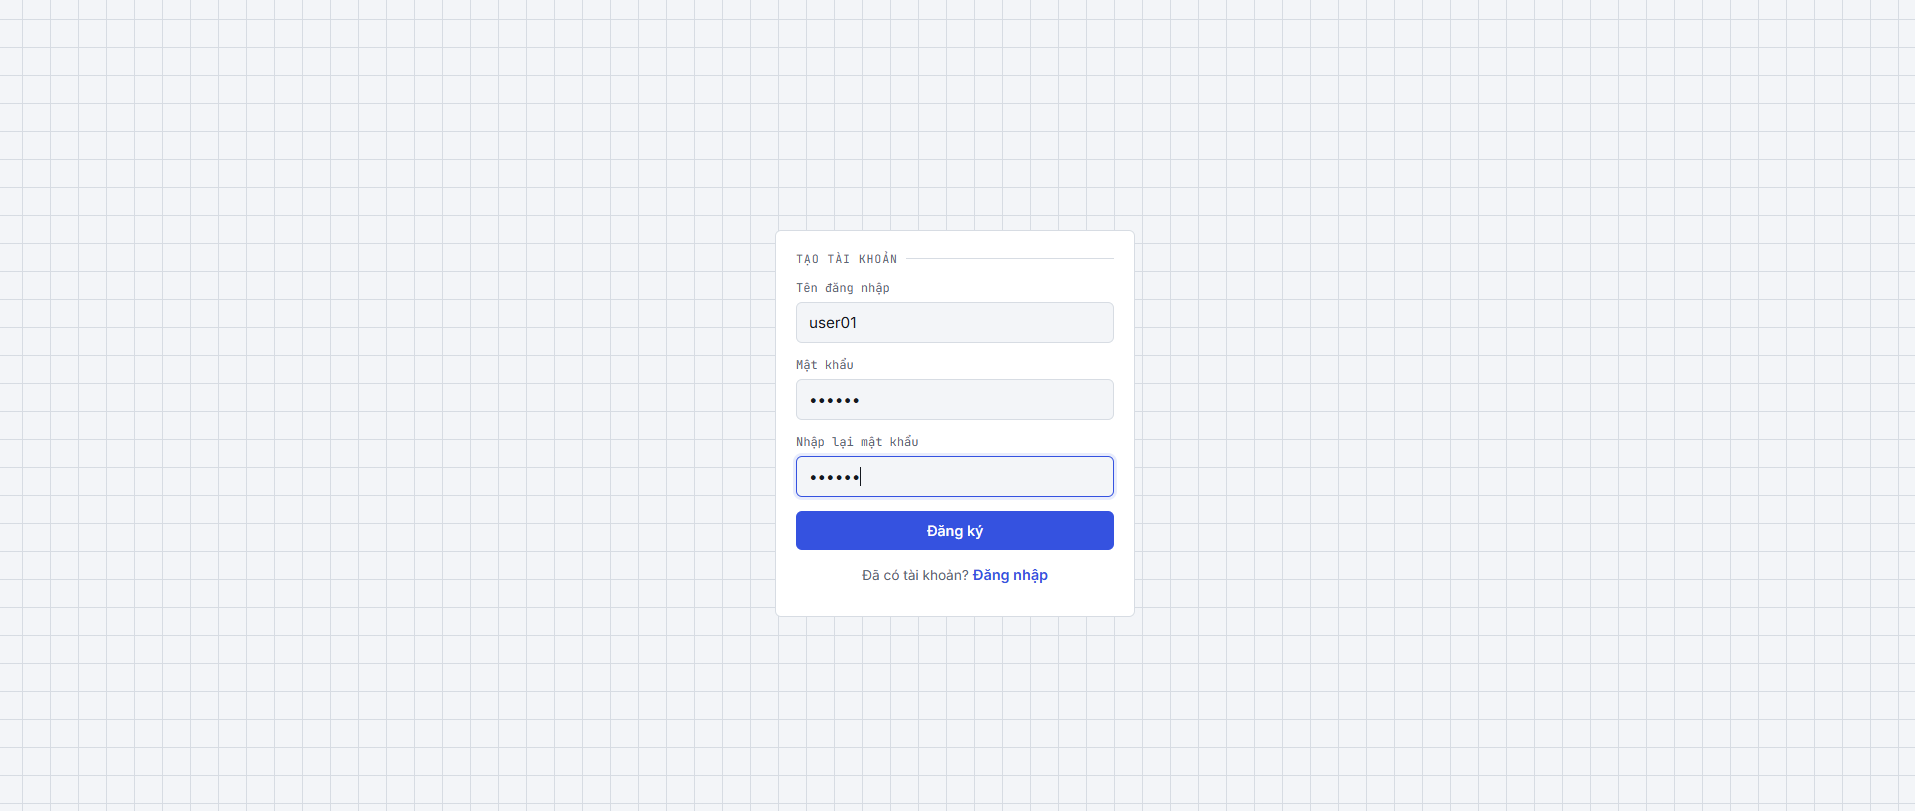
\includegraphics[width=1.0\textwidth]{images/chapter_03/img_26.png}
    \caption{Giao diện đăng ký tài khoản}
    \label{fig:nlp}
\end{figure}

\subsection{Giao diện đăng nhập}
\begin{figure}[H]
    \centering
    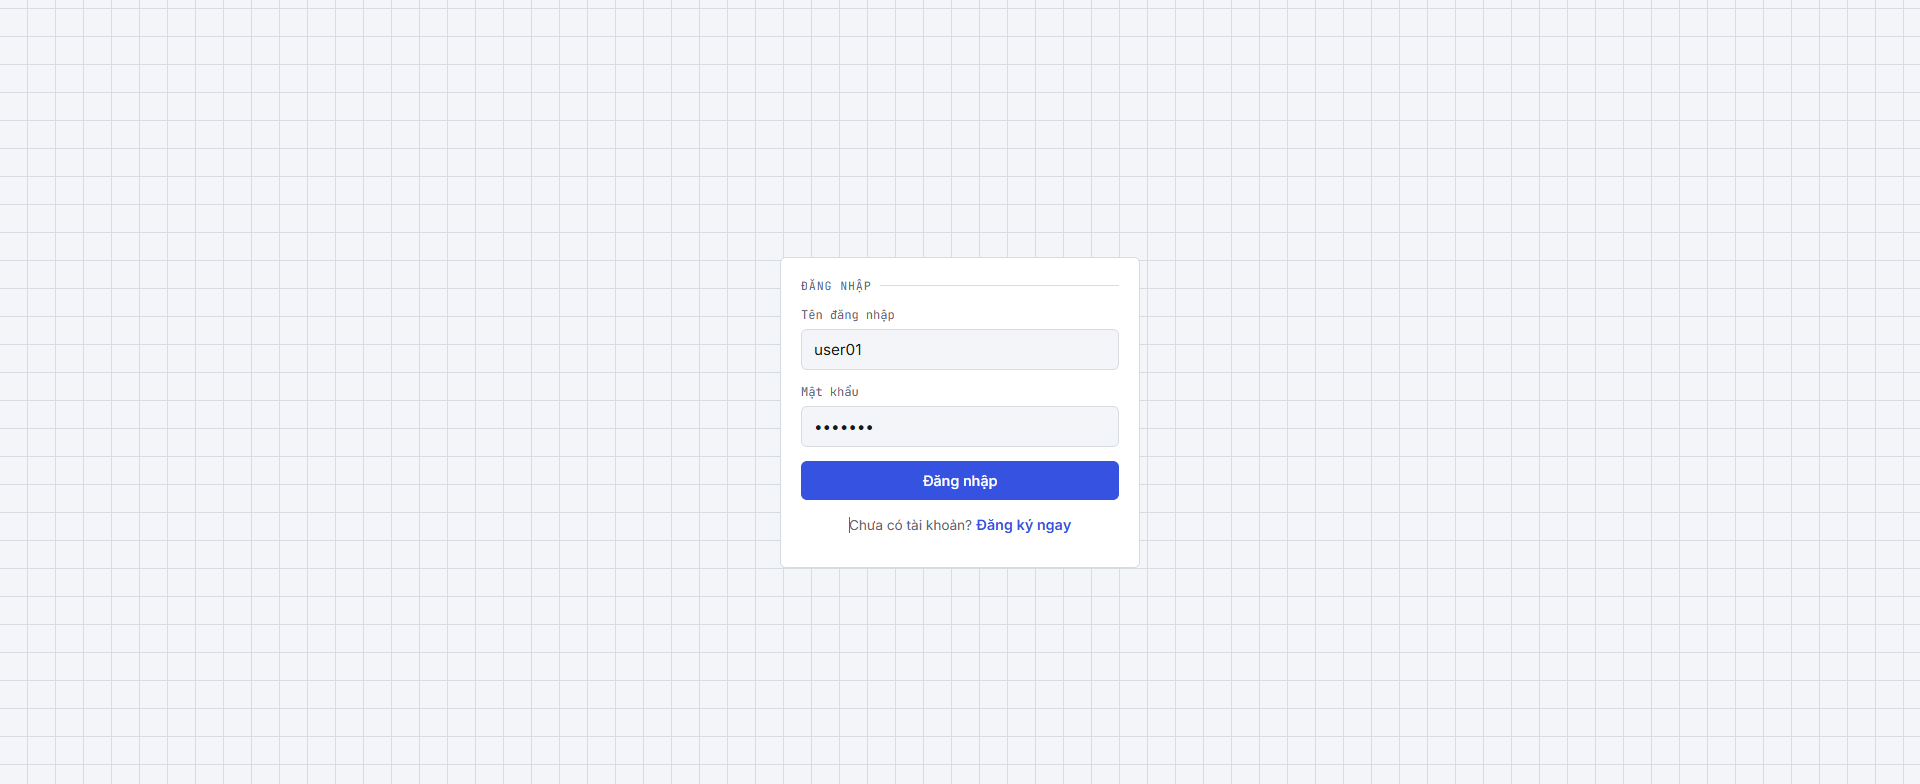
\includegraphics[width=1.0\textwidth]{images/chapter_03/img_27.png}
    \caption{Giao diện đăng nhập tài khoản}
    \label{fig:nlp}
\end{figure}

\subsection{Giao diện trang chủ}
\begin{figure}[H]
    \centering
    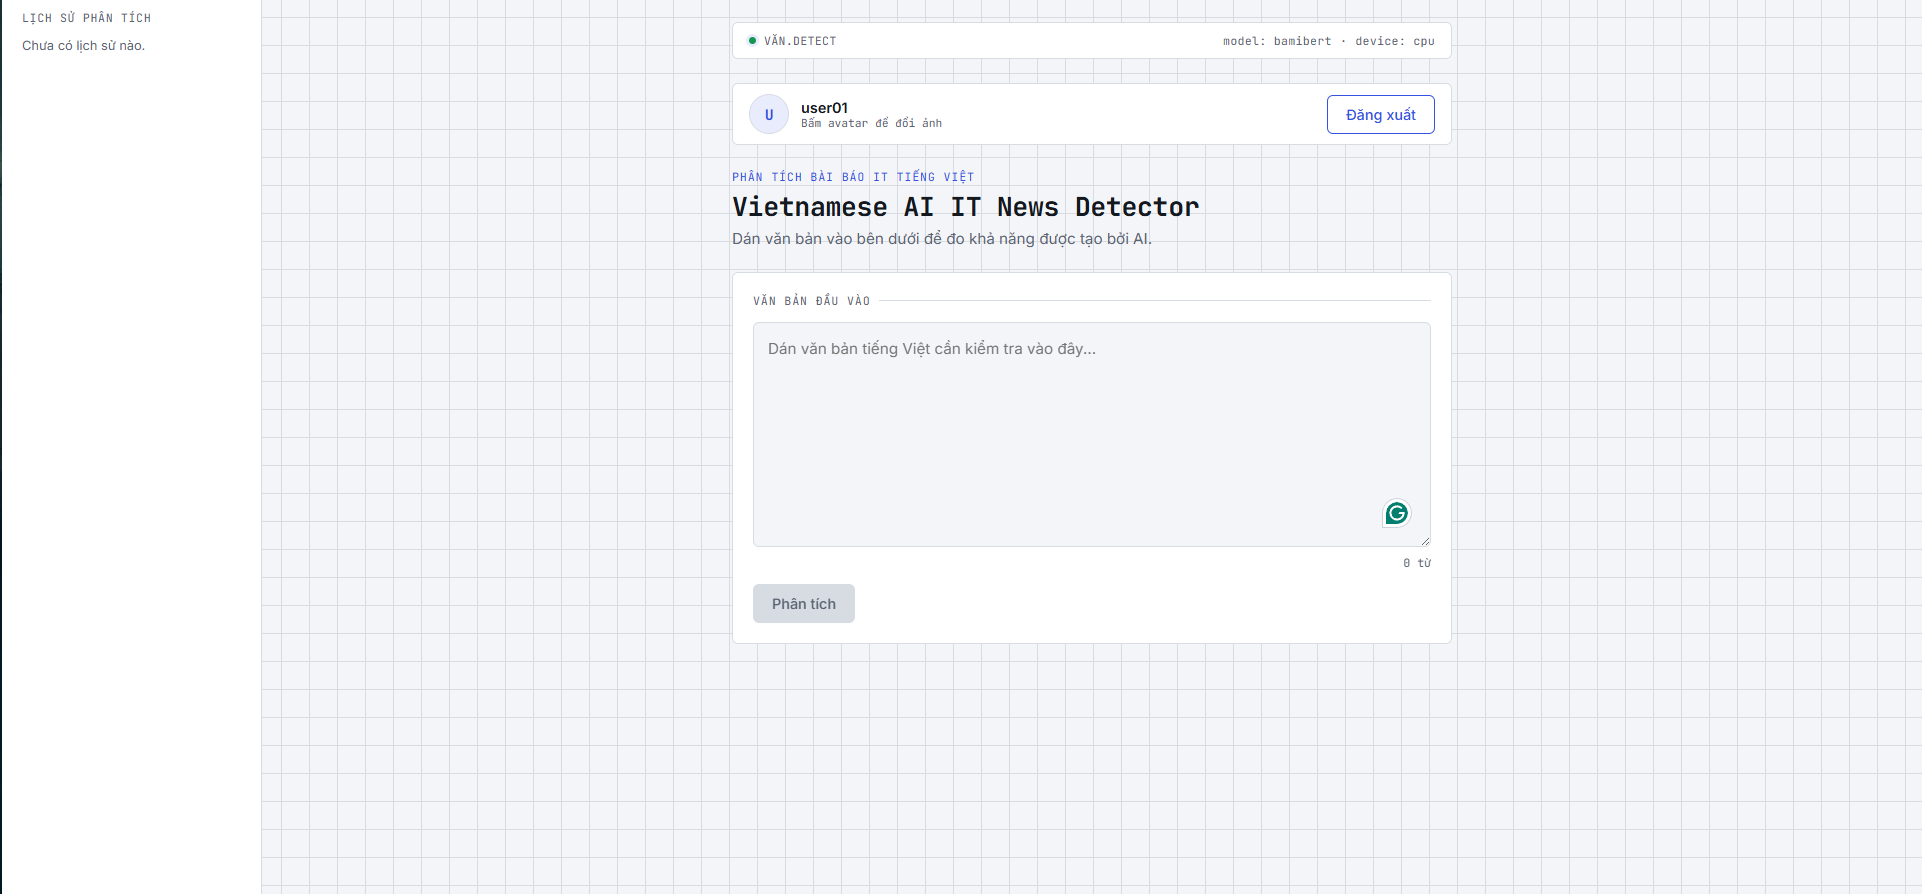
\includegraphics[width=1.0\textwidth]{images/chapter_03/img_28.png}
    \caption{Giao diện trang chủ}
    \label{fig:nlp}
\end{figure}

\subsection{Giao diện dự đoán}
\begin{figure}[H]
    \centering
    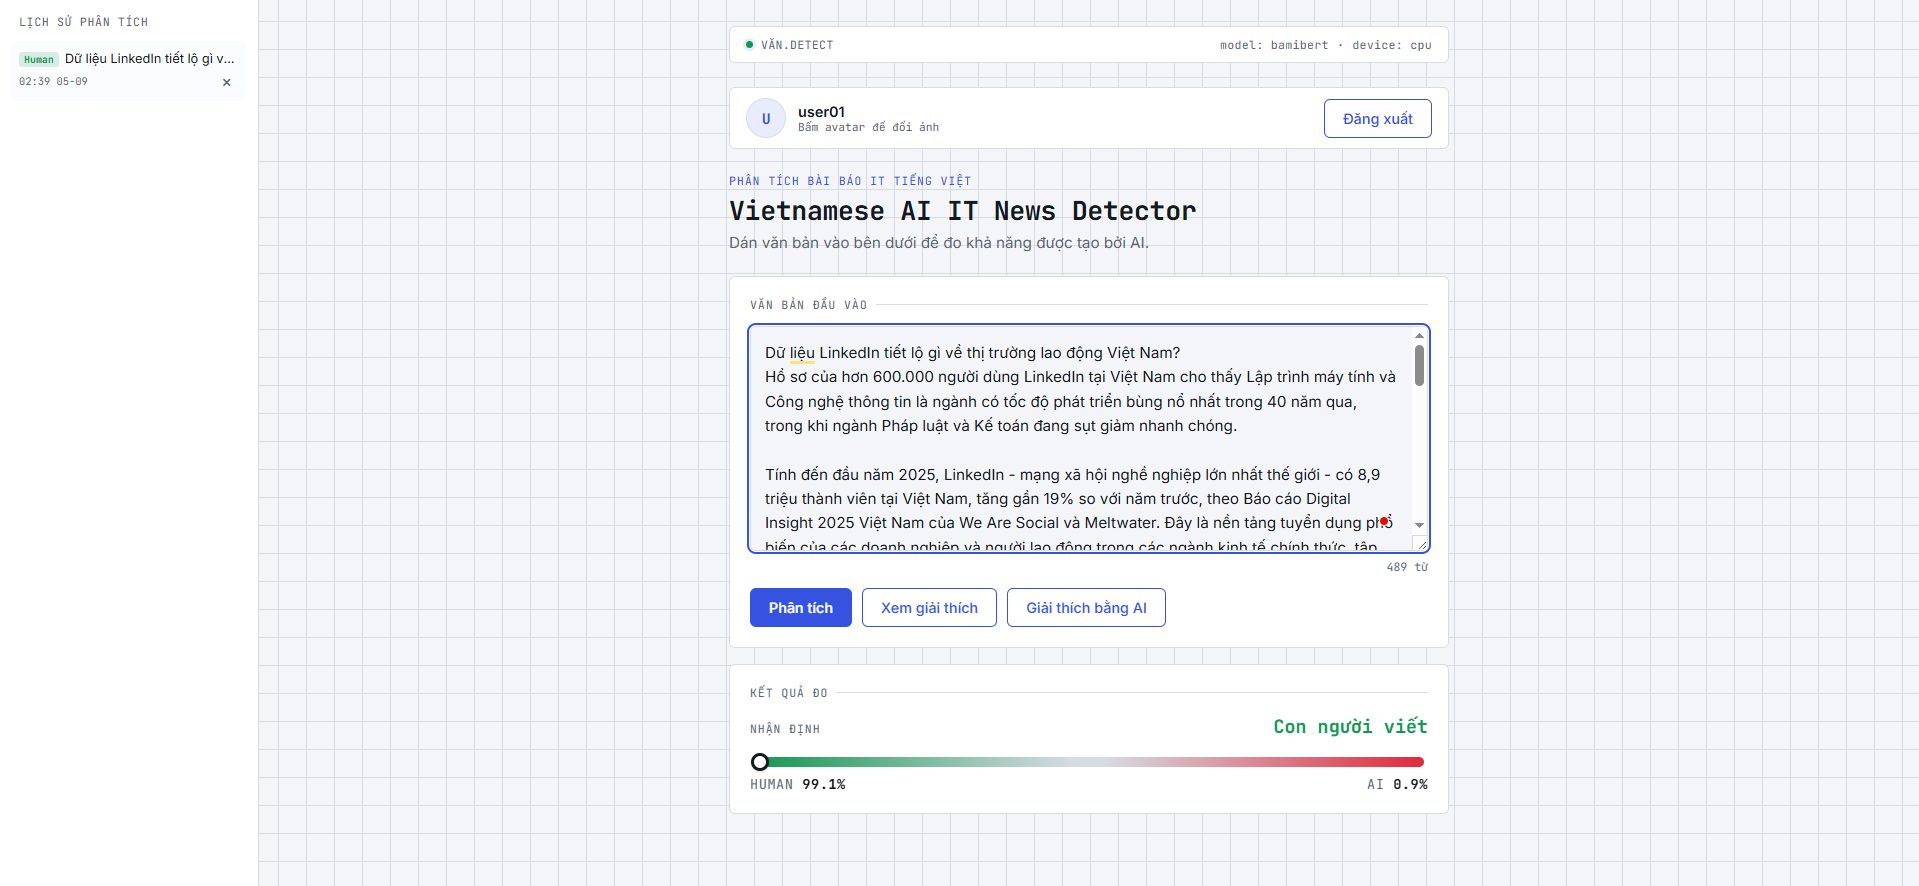
\includegraphics[width=1.0\textwidth]{images/chapter_03/img_29.png}
    \caption{Giao diện dự đoán}
    \label{fig:nlp}
\end{figure}

\subsection{Giao diện lịch sử}
\begin{figure}[H]
    \centering
    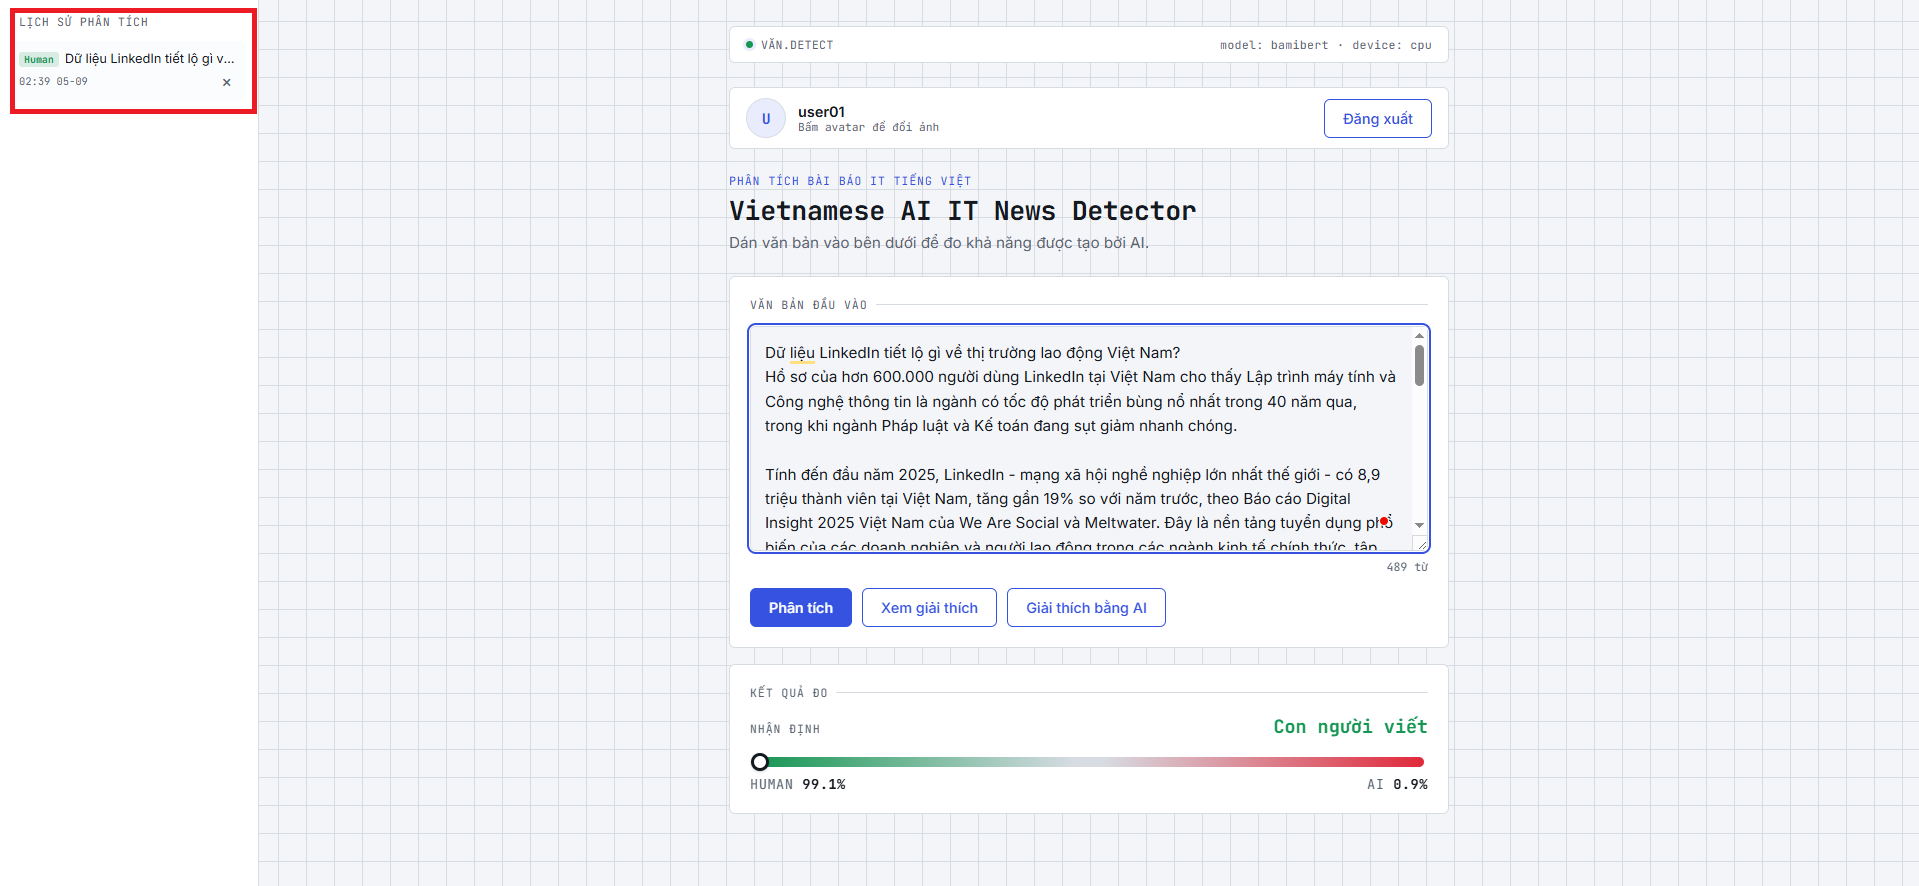
\includegraphics[width=1.0\textwidth]{images/chapter_03/img_30.png}
    \caption{Giao diện hiển thị lịch sử}
    \label{fig:nlp}
\end{figure}

\subsection{Giao diện giải thích highlight text}
\begin{figure}[H]
    \centering
    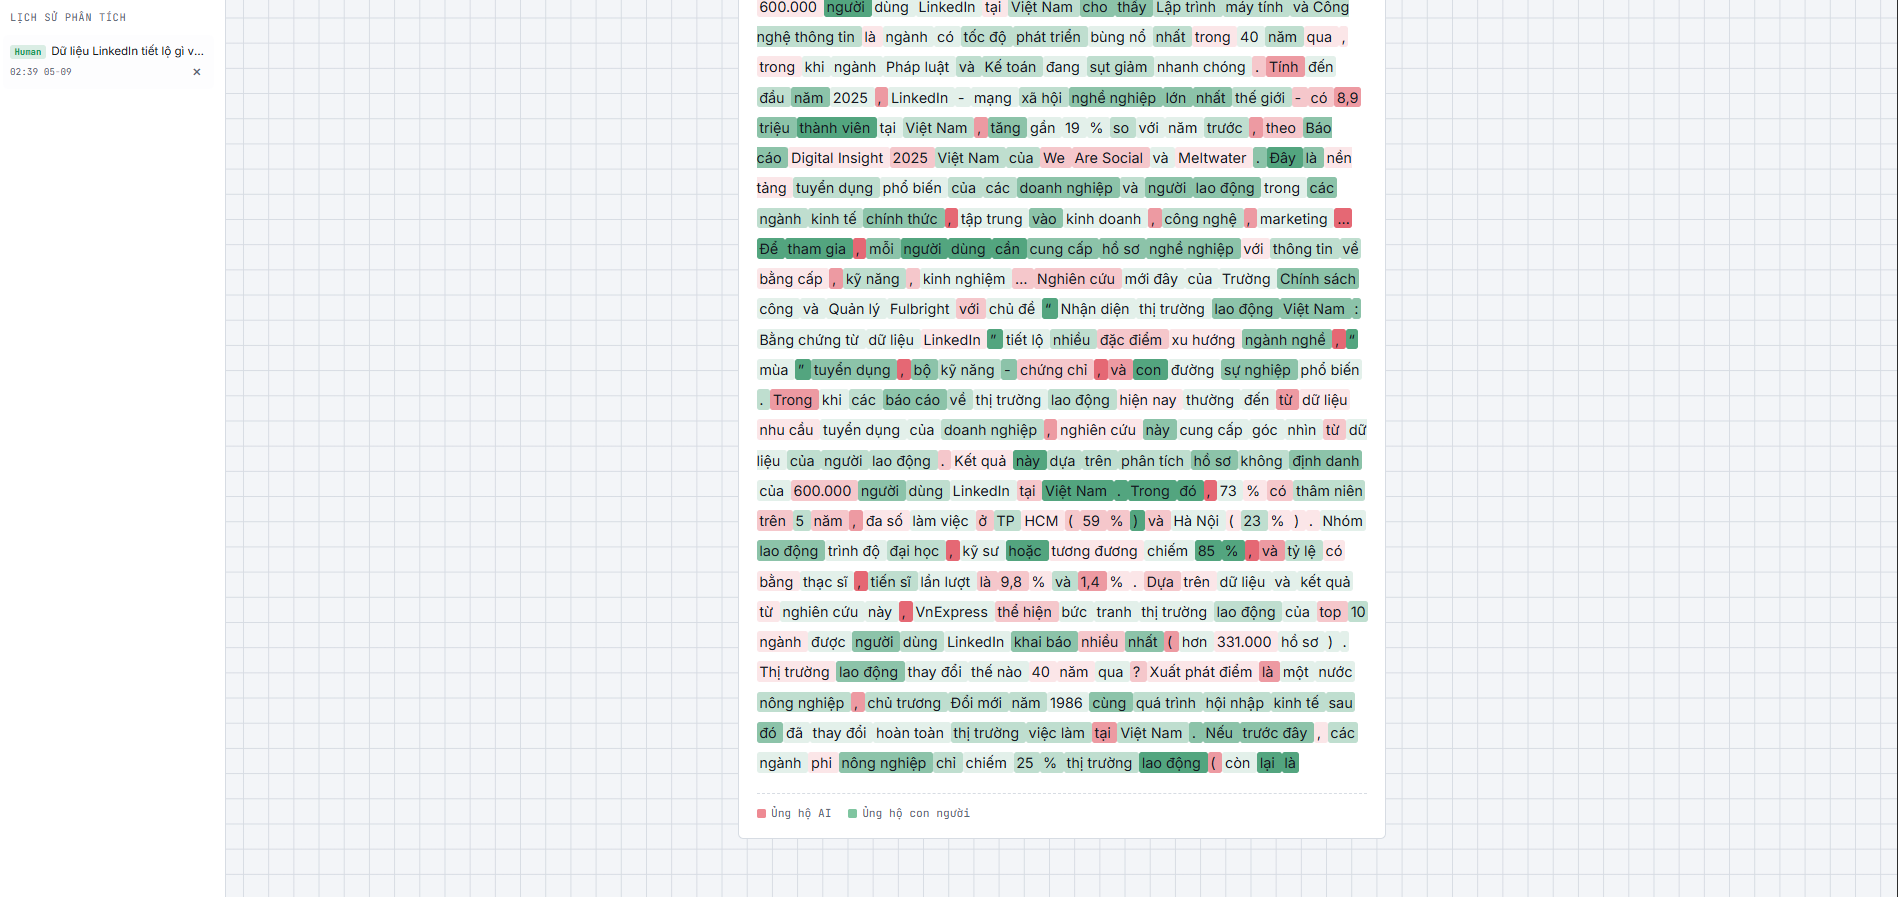
\includegraphics[width=1.0\textwidth]{images/chapter_03/img_31.png}
    \caption{Giao diện hiển thị text highlight}
    \label{fig:nlp}
\end{figure}

\subsection{Giao diện giải thích bằng LLM}
\begin{figure}[H]
    \centering
    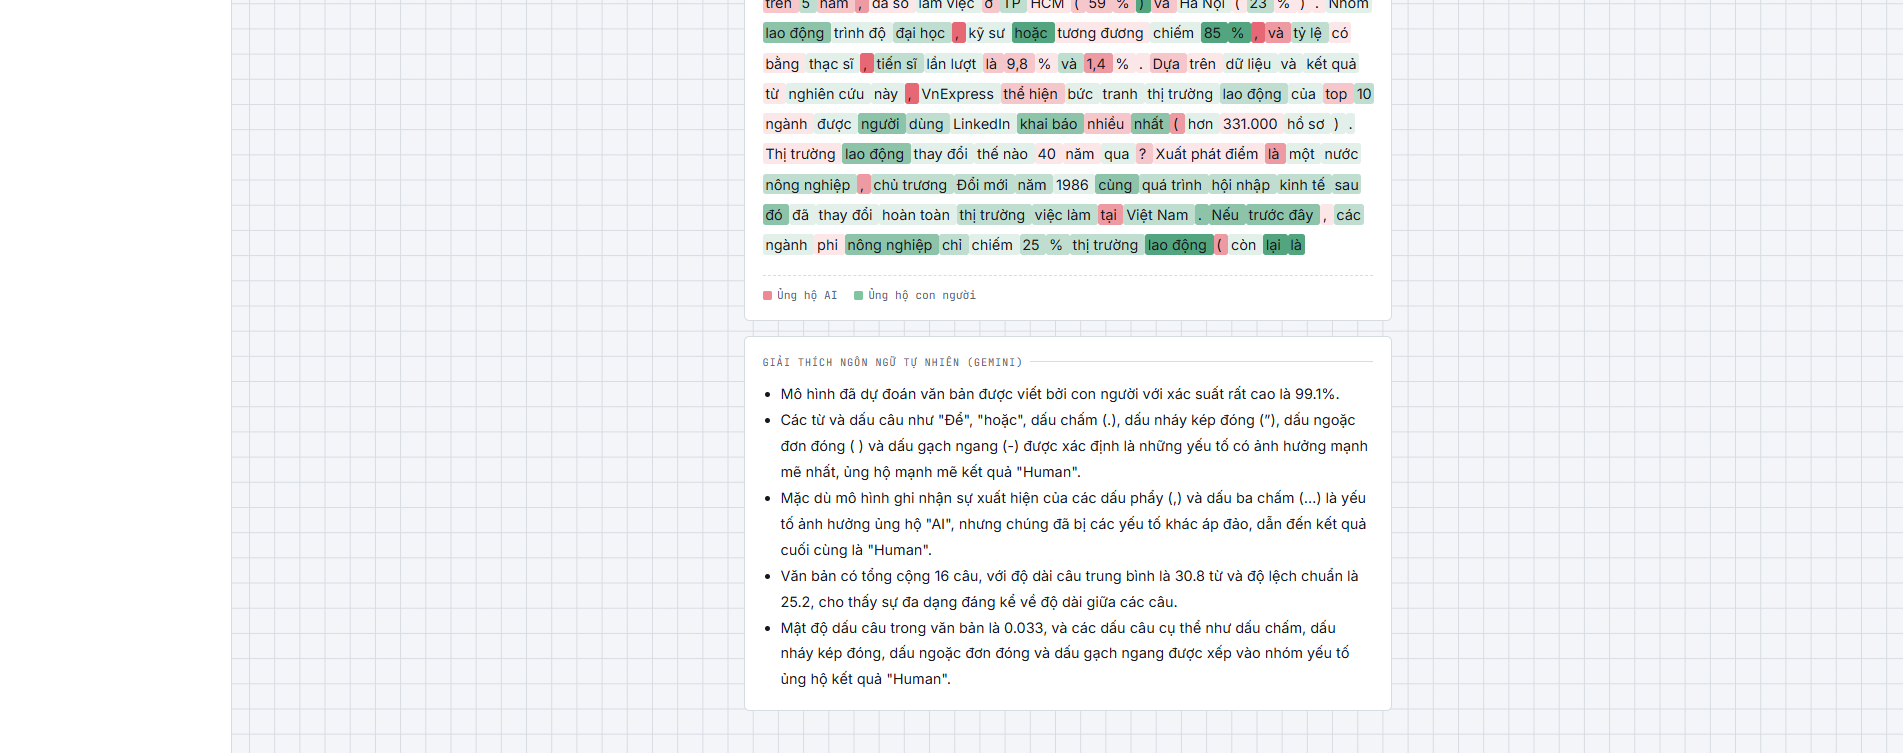
\includegraphics[width=1.0\textwidth]{images/chapter_03/img_32.png}
    \caption{Giao diện hiển thị kết quả giải thích LLM}
    \label{fig:nlp}
\end{figure}